\documentclass[11pt]{article}

\usepackage[margin=1in]{geometry}
\usepackage[T1]{fontenc}
\usepackage[utf8]{inputenc}
\usepackage{amsmath,amssymb}
\usepackage{booktabs}
\usepackage{array}
\usepackage{graphicx}
\usepackage{subcaption}
\usepackage{float}
\usepackage[section]{placeins}
\usepackage{hyperref}

\hypersetup{
    colorlinks=true,
    linkcolor=blue,
    citecolor=blue,
    urlcolor=blue
}

\title{\textbf{Adaptive Preconditioned Dynamics, Solution Geometry, and Generalization in Neural Networks}\\
\Large A Matched-Seed Study of SGD and Adam Across Parameter, Basin, Function, and Representation Geometry}
\author{Changyuan Yu(cy2812)~~~~~Xiangyu Liao(xl3581)\\Zhiliang Wang(zw3162)~~~~~Kevin Sun(ys3978)}
\date{May 2026}

\begin{document}
\maketitle

\begin{abstract}
When we think about adaptive optimizers, we often see them as a way to speed up the learning process. However, in complex neural networks, they can also influence which solution is chosen, even if both solutions have similar performance. To better understand this, we compare two popular optimizers, SGD with momentum and Adam, under a matched-seed protocol on Fashion-MNIST. From a mathematical perspective, SGD applies a simple scalar preconditioning, whereas Adam uses a time-varying diagonal preconditioner; this difference shapes how the local error dynamics evolve. Our analysis is organized around three project questions: \emph{convergence}, \emph{solution geometry}, and \emph{generalization}. For solution geometry we test the optimizer-induced effect with six complementary measurements (distance from initialization, trajectory path length and update norm, Hessian sharpness/trace, perturbation flatness, inter-seed dispersion, and a loss-matched control), so that no single proxy carries the conclusion. For generalization we follow the resulting parameter-space difference through three additional levels of geometry: basin connectivity (linear mode connectivity), function-space agreement (prediction disagreement, symmetric KL, logit cosine), and representation alignment (linear CKA). Adam moves substantially farther from the starting point and selects more dispersed solutions, and on the MLP it lands in distinctly flatter regions even after loss matching. Despite this, the differences shrink as the comparison propagates: matched-seed cross-optimizer basin barriers are an order of magnitude smaller than same-optimizer cross-seed barriers, prediction disagreement and CKA fall within the same-optimizer cross-seed baseline, and only logit-direction cosine still shows a sharp cross-optimizer signal. The implicit bias of Adam vs.\ SGD is therefore real at the parameter level but is filtered through architecture, basin connectivity, and representation alignment before it reaches generalization.
\end{abstract}

\section{Introduction}

Today's neural networks usually have way too many parameters, which means they can learn the training data in lots of different ways. Often, many of these ways can get really close to perfect accuracy on the training data. When this happens, the optimizer's job isn't just to minimize the error on the training data. It also plays a role in choosing which of these many possible solutions the training process actually ends up with. This effect of the optimizer on the solution is often referred to as the ``implicit bias'' or ``implicit regularization'' of the algorithm. In simpler terms, the optimizer is not just finding the best fit, but also influencing which of the many good fits is chosen. This can have a big impact on how well the neural network works in practice.

Here we ask whether adaptive optimizers change that implicit bias. We focus on the comparison between SGD with momentum and Adam. SGD applies one global learning-rate scale to all coordinates of the stochastic gradient. Adam instead rescales each coordinate using estimates of the first and second moments of recent gradients \cite{kingma2015adam}. This coordinate-wise adaptation is often helpful in early optimization, especially when gradients vary strongly across layers or coordinates. At the same time, it may also change the geometry of the final solution and therefore affect generalization.

The overall project question is: \begin{quote} \emph{Do adaptive optimizers alter the implicit bias and generalization of neural networks?} \end{quote} We organize the entire study around three linked sub-questions: \begin{enumerate} \item \textbf{Early-stage convergence.} Does Adam converge faster than SGD at the beginning of training? \item \textbf{Solution geometry.} If Adam is faster, does it reach a different kind of solution, or only the same solution earlier? \item \textbf{Generalization.} Do the observed geometric differences explain differences in test performance and train--test gap? \end{enumerate} These three questions form the spine of the report. They are not investigated with a single proxy each, however: the geometry question is tested with six complementary measurements (distance from initialization, cumulative path length and per-step update norm, Hessian sharpness/trace, isotropic perturbation flatness, inter-seed parameter dispersion, and a loss-matched control), so that no single quantity carries the verdict. The generalization question is then traced through three additional levels of geometry that probe how a parameter-space difference can or cannot become a generalization difference: basin connectivity along the linear interpolant between two trained solutions, function-space agreement on test predictions, and representation alignment in penultimate-layer features. The contributions are accordingly: \begin{enumerate} \item We formulate SGD and Adam as two preconditioned stochastic dynamics and develop a local quadratic analysis $e_{t+1}\approx (I-P_tH)e_t$ that explains why a time-varying diagonal preconditioner can change the selected low-loss solution. \item We use matched seeds (shared initialization, shared minibatch order) to isolate optimizer-induced effects from initialization and batch-order randomness, and add a same-optimizer cross-seed baseline as a falsification test. \item We characterize the geometry question with six complementary diagnostics (distance, path length and update norm, Hessian curvature proxies, isotropic perturbation flatness, inter-seed dispersion, and a loss-matched checkpoint comparison) so that the geometry verdict does not depend on a single proxy. \item We trace the generalization question through three further levels: linear mode connectivity tests whether two trained solutions share a basin; prediction disagreement, symmetric KL and logit cosine test whether they realize the same predictor; and feature-kernel alignment plus linear CKA test whether they share representations. We organize the resulting evidence into a three-level synthesis: parameter, basin, and function--representation geometry. \end{enumerate}

The answer is not simply that Adam is better or worse than SGD. Instead, the experiments show a conditional pattern. In the MLP, Adam has a clear early optimization advantage and lands in much flatter solutions according to the Hessian proxies we measure ($5\times$ lower $\lambda_{\max}$, $6\times$ lower trace), and this flatness gap survives the loss-matched control. Even so, these geometric differences do not produce a clear generalization advantage: test accuracy and train--test gap differ by less than the observed seed-to-seed variation, which is not fully explained by a naive flat-minima interpretation. In the CNN, Adam is still slightly faster in training loss, but its dominant Hessian eigenvalue is actually higher than SGD's, while both optimizers reach similar test accuracy and generalization gaps. In other words, adaptive optimization changes the training trajectory and the selected parameter region, but whether this geometric change matters for generalization depends on architecture, on whether the two endpoints share a basin, and on how much of the parameter difference survives at the predictor and representation levels.

\subsection{Scope of Claims}

The implicit-bias and generalization claims in this report are claims about Adam-vs-SGD trajectory and solution geometry \emph{at the scale and protocol of this study}: small image-classification architectures on Fashion-MNIST under a matched-seed protocol with no explicit regularization, trained for tens of epochs across a handful of seeds. The MLP/SmallCNN architecture pair is a controlled scale-down designed to expose mechanism, not a representative sample of modern deep learning. We do not claim that the same effects, in the same direction or magnitude, transfer to large-scale settings such as ResNets on ImageNet, transformer language models, or training horizons of $10^4$+ steps. The full experimental protocol is given in Section~\ref{sec:setup} and a detailed list of caveats appears in Section~\ref{sec:limitations}.


\section{Mathematical Background and Problem Description}

Let $\widehat L(\theta)$ denote the empirical cross-entropy loss and let
\[
g_t=\nabla_\theta \widehat L_{B_t}(\theta_t)
\]
be the stochastic gradient on minibatch $B_t$. Rather than treating SGD and Adam as two unrelated engineering rules, we view both as preconditioned stochastic dynamics,
\[
\theta_{t+1}=\theta_t-P_t q_t,
\]
where $q_t$ is a gradient-like direction and $P_t$ is the effective preconditioner.
For SGD with momentum,
\[
u_t=\mu u_{t-1}+g_t,\qquad \theta_{t+1}=\theta_t-\eta u_t,
\]
so momentum smooths gradients over time, while the spatial scaling remains scalar: $P_t=\eta I$. Expanding the recursion,
\[
u_t=\sum_{k=0}^t \mu^{t-k}g_k,
\]
shows that momentum is a temporal averaging mechanism, not a coordinate-wise metric change.

Adam instead computes
\[
m_t=\beta_1m_{t-1}+(1-\beta_1)g_t,\qquad
v_t=\beta_2v_{t-1}+(1-\beta_2)g_t^{\odot 2},
\]
with bias-corrected moments
\[
\hat m_t=\frac{m_t}{1-\beta_1^t},\qquad
\hat v_t=\frac{v_t}{1-\beta_2^t}.
\]
Its update can be written as
\[
\theta_{t+1}=\theta_t-\alpha\frac{\hat m_t}{\sqrt{\hat v_t}+\varepsilon}
=\theta_t-\alpha D_t\hat m_t,
\]
where
\[
D_t=\operatorname{diag}\!\left(\frac{1}{\sqrt{\hat v_{t,i}}+\varepsilon}\right)_i.
\]
Thus the key mathematical contrast is scalar spatial preconditioning for SGD versus time-varying diagonal preconditioning for Adam.

This distinction matters in local geometry. Near a low-loss point $\theta^\star$, approximate
\[
\widehat L(\theta)\approx \widehat L(\theta^\star)+\frac12(\theta-\theta^\star)^\top H(\theta-\theta^\star).
\]
For $e_t=\theta_t-\theta^\star$, preconditioned gradient dynamics obey
\[
e_{t+1}\approx (I-P_tH)e_t.
\]
For SGD, this becomes $e_{t+1}\approx (I-\eta H)e_t$. If $H=Q\Lambda Q^\top$ and $\tilde e_t=Q^\top e_t$, then
\[
\tilde e_{t+1,i}=(1-\eta\lambda_i)\tilde e_{t,i}.
\]
A single scalar learning rate controls all Hessian eigendirections. For Adam, however,
\[
e_{t+1}\approx (I-\alpha D_tH)e_t,
\]
and $D_t$ generally does not commute with $H$. In the Hessian eigenbasis,
\[
\tilde e_{t+1}=\bigl(I-\alpha Q^\top D_tQ\Lambda\bigr)\tilde e_t,
\]
which can mix eigendirections. Equivalently, Adam responds to an effective preconditioned curvature
\[
H_t^{\mathrm{eff}}=D_t^{1/2}HD_t^{1/2}.
\]
This is the central reason Adam should not be interpreted merely as a faster clock for SGD.

In an over-parameterized network, the low-loss set
\[
\mathcal S_\varepsilon=\{\theta:\widehat L(\theta)\le \varepsilon\}
\]
contains many parameter vectors. The optimizer acts as a selection map
\[
\theta^\star_{\mathcal A}=A_{\mathcal A}(\theta_0,\{B_t\},\text{hyperparameters}).
\]
Our matched-seed protocol compares $\theta^\star_{\mathrm{SGD}}$ and $\theta^\star_{\mathrm{Adam}}$ under identical initialization and minibatch order, so observed differences are more directly attributable to the update rule.

We use Hessian quantities as local geometry diagnostics. The dominant curvature is
\[
\lambda_{\max}(H)=\max_{\|u\|_2=1}u^\top Hu,
\]
and the aggregate curvature is $\operatorname{tr}(H)=\sum_i\lambda_i(H)$. For a small perturbation,
\[
\Delta\widehat L(\delta)\approx \frac12\delta^\top H\delta.
\]
If $\delta\sim\mathcal N(0,\sigma^2I)$, then
\[
\mathbb E[\Delta\widehat L(\delta)]\approx \frac{\sigma^2}{2}\operatorname{tr}(H).
\]
This identity motivates the perturbation-flatness measurement that complements the Hessian proxies in Section~\ref{sec:perturbation}.

Finally, sharpness must be interpreted carefully. Euclidean Hessian spectra are parameter-space diagnostics, not invariant measures of function complexity. For ReLU networks, rescaling one layer and inversely rescaling the next can leave the represented function unchanged while changing parameter norms and curvature. Therefore our Hessian and perturbation metrics are used as controlled within-protocol diagnostics, and we later test whether parameter differences survive in basin, function, and representation space.

\subsection{Project Hypotheses}

We test three linked hypotheses. First, Adam should reduce training loss faster than default SGD because diagonal preconditioning adapts coordinate-wise step scales. Second, Adam and SGD should select different parameter-space regions even under matched initialization and minibatch order, and this difference should be observable on multiple complementary geometry diagnostics rather than a single proxy. Third, parameter-space geometry alone should not fully determine generalization; the parameter-level difference is filtered, in turn, through architecture, basin connectivity, function-space behavior, and representation similarity.

\section{Experimental Setup}
\label{sec:setup}

All experiments use Fashion-MNIST with the standard train/test split and normalized grayscale inputs. We compare two architectures: a batch-normalized MLP and a SmallCNN with two convolutional blocks followed by a small classifier. The MLP has weaker image-specific inductive bias, so optimizer-induced effects should be easier to observe; the CNN adds convolution, pooling, and weight sharing, allowing us to test whether architecture compresses optimizer differences.

The main experiments use five seeds, $\{42,123,456,789,2024\}$. For each seed, the SGD and Adam runs start from the same initialization and use the same deterministic data-loader shuffle. The main protocol uses no weight decay, dropout, or data augmentation, so that explicit regularization does not obscure optimizer-induced effects.

\begin{table}[H]
\centering
\begin{tabular}{ll}
\toprule
\textbf{Component} & \textbf{Setting}\\
\midrule
Dataset & Fashion-MNIST\\
Batch size & 128\\
Epochs & 30\\
Loss & Cross-entropy\\
Seeds & 42, 123, 456, 789, 2024\\
SGD & learning rate 0.01, momentum 0.9, weight decay 0\\
Adam & learning rate 0.001, betas $(0.9,0.999)$, weight decay 0\\
Architectures & Batch-normalized MLP and SmallCNN\\
\bottomrule
\end{tabular}
\caption{Main experimental protocol.}
\label{tab:setup}
\end{table}

The measured quantities are organized by which of the three project questions they answer. \emph{Convergence} (Part~I): training-loss curves and threshold crossing. \emph{Solution geometry} (Part~II): six complementary measurements --- distance from initialization, cumulative path length and per-step update norm, Hessian sharpness/trace, isotropic perturbation flatness, inter-seed parameter dispersion, and a loss-matched checkpoint comparison. \emph{Generalization} (Part~III): test accuracy and train--test gap, plus three further levels of geometry (linear mode connectivity, function-space disagreement, representation-space CKA) that test how a parameter-space difference propagates to predictions.

\section{Part I: Early-Stage Convergence}

Adam's most immediate expected advantage is faster early training. We therefore record the first global step at which each run crosses fixed training-loss thresholds. This section is mainly motivational: the deeper question is not whether Adam reaches low loss earlier, but whether it selects a different solution once low loss is reached.

\begin{table}[H]
\centering
\begin{tabular}{llrrrr}
\toprule
\textbf{Model} & \textbf{Threshold} & \textbf{SGD steps} & \textbf{SGD std} & \textbf{Adam steps} & \textbf{Adam std}\\
\midrule
MLP & 2.0 & 5.4 & 0.5 & 2.6 & 0.5\\
MLP & 1.0 & 12.8 & 1.9 & 6.8 & 0.8\\
MLP & 0.5 & 54.2 & 1.3 & 30.8 & 4.6\\
MLP & 0.2 & 643.2 & 137.7 & 477.0 & 96.7\\
\midrule
SmallCNN & 2.0 & 4.4 & 0.5 & 3.8 & 0.8\\
SmallCNN & 1.0 & 9.4 & 2.1 & 8.8 & 1.5\\
SmallCNN & 0.5 & 36.8 & 9.4 & 32.2 & 5.1\\
SmallCNN & 0.2 & 346.8 & 38.9 & 312.2 & 49.6\\
\bottomrule
\end{tabular}
\caption{Mean global steps to first reach each training-loss threshold across five seeds. Lower is faster.}
\label{tab:q1_thresholds}
\end{table}

Adam reaches every threshold earlier on average. The effect is strongest in the MLP: for the strict threshold $0.2$, Adam requires $477.0$ steps while SGD requires $643.2$ steps. In the CNN, Adam is still faster, but the gap is smaller because both optimizers fit the architecture well. A small learning-rate check on the MLP shows that tuned SGD can narrow parts of this early gap, so we do not claim Adam is universally faster. The defensible conclusion is narrower: Adam is faster than the default SGD baseline under the matched protocol, especially in the MLP. This motivates the next question: does Adam merely arrive earlier, or does it arrive at a different kind of solution?

\FloatBarrier

\section{Part II: Solution Geometry --- Multi-Faceted Evidence}
\label{sec:part2}

\subsection{Question and Roadmap}

The second project question asks whether Adam and SGD converge to geometrically different solutions, or whether Adam simply arrives at the same kind of solution faster. We answer this with six complementary measurements, organized so that each addresses a distinct way the question could be wrong:
\begin{enumerate}
\item Distance from initialization (Section~\ref{sec:dist}) measures the net displacement of each optimizer from $\theta_0$.
\item Trajectory decomposition (Section~\ref{sec:path-length}) splits that displacement into cumulative path length, directness ratio, and per-step update norm, distinguishing ``Adam moves farther because it takes larger steps'' from ``Adam follows a more directed drift.''
\item Hessian curvature (Section~\ref{sec:hessian}) probes the shape of the loss surface around each endpoint via $\lambda_{\max}(H)$ and $\operatorname{tr}(H)$.
\item Perturbation flatness (Section~\ref{sec:perturbation}) operationalizes the Hessian proxies by directly measuring the loss increase under controlled isotropic perturbations.
\item Inter-seed parameter dispersion (Section~\ref{sec:dispersion}) checks whether each optimizer reproducibly lands in similar regions or in scattered ones.
\item Loss-matched control (Section~\ref{sec:loss-matched}) rules out the possibility that the geometric differences are simply an artifact of comparing endpoints at different training-loss levels.
\end{enumerate}
A summary of the combined evidence appears in Section~\ref{sec:part2-synthesis}. Throughout this part, the same five matched seeds are used, so geometric differences are not driven by initialization or minibatch order.

\subsection{Distance from Initialization}
\label{sec:dist}

\begin{figure}[H]
\centering
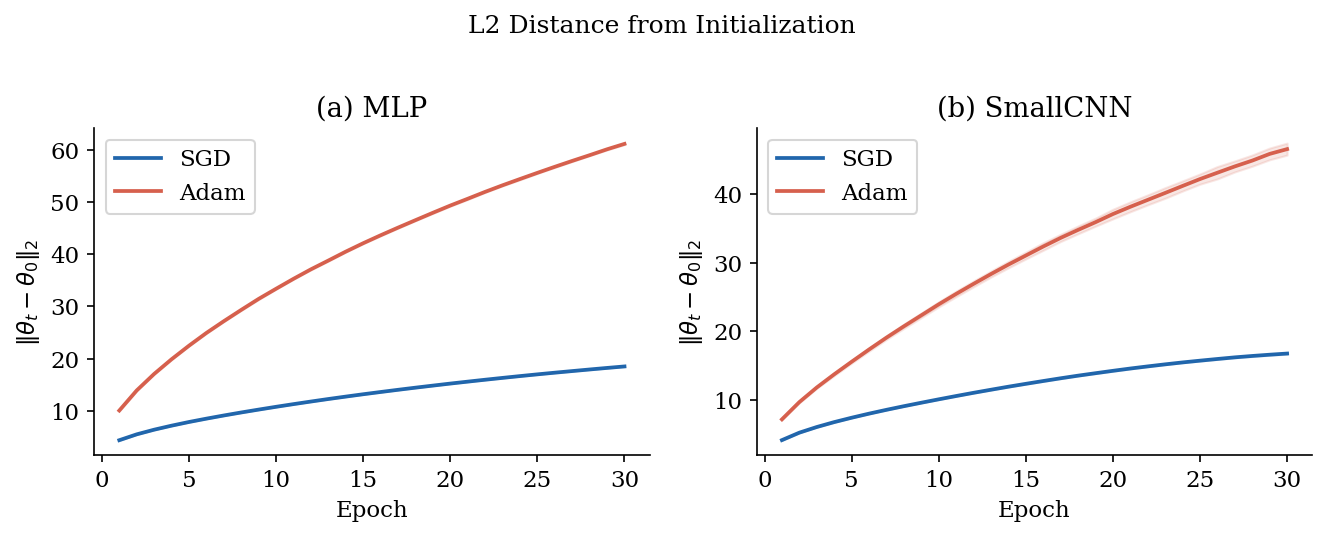
\includegraphics[width=\linewidth]{figures/part2_geometry/param_distance.png}
\caption{L2 distance from initialization $\|\theta_t - \theta_0\|_2$ over training epochs.
  Shaded bands show $\pm 1$ standard deviation across five matched seeds.
  Adam moves substantially farther from the starting point in both architectures,
  and its trajectory is concave (fast early, decelerating later) while SGD drifts linearly.}
\label{fig:param_distance}
\end{figure}

Figure~\ref{fig:param_distance} shows how far each optimizer moves from the shared initialization $\theta_0$.
In the MLP, Adam reaches a final parameter distance of $61.20 \pm 0.15$, while SGD reaches only $18.49 \pm 0.03$, a factor of $3.3\times$.
In the SmallCNN, Adam reaches $46.79 \pm 0.94$ while SGD reaches $16.75 \pm 0.09$, a factor of $2.8\times$.
Both differences are well outside seed-to-seed variation.

The shapes of the trajectories are qualitatively distinct. Adam's curve is concave: it advances rapidly in the first five epochs and then decelerates, while SGD follows a more linear drift throughout. This concave trajectory is consistent with Adam's adaptive preconditioning,
\[
  \eta^{\mathrm{Adam}}_{t,i} = \frac{\alpha}{\sqrt{\hat{v}_{t,i}} + \varepsilon},
\]
and with the changing gradient statistics during training. We should not interpret the curve as evidence for one single mechanism, but it does show that Adam and SGD are not simply following the same path at different speeds. Since both optimizers share identical $\theta_0$ and data ordering, the large distance difference is most naturally explained by the optimizer update rule.

At the same time, this is a parameter-space statement rather than a direct function-space statement. Neural networks can represent similar functions with different parameter vectors, especially in the presence of scaling symmetries and BatchNorm. Therefore, distance from initialization shows that the optimizer trajectories and selected parameter regions differ, but it does not by itself prove that the learned input--output functions differ by the same amount; this is examined in Section~\ref{sec:function-space}.

\paragraph{Why not raw gradient norm.} We do not use raw gradient norm as evidence of flatness, because Adam updates preconditioned gradients rather than raw gradients. The more relevant trajectory diagnostics are actual parameter movement: net distance here, and cumulative path length and per-step update norm in Section~\ref{sec:path-length}.

\subsection{Trajectory Decomposition: Path Length and Update Norm}
\label{sec:path-length}

The previous subsection establishes that Adam ends up at a point much farther from $\theta_0$ than SGD does. By itself this only describes the \emph{net} displacement. Two trajectories can have the same endpoint distance while traversing very different routes. To distinguish ``Adam moves farther because it takes larger steps'' from ``Adam follows a more directed drift,'' we now record the \emph{cumulative} parameter movement and the per-step update norm.

\paragraph{Cumulative path length.} For a training run with $T$ minibatch updates, define
\[
\mathcal{P}_T
= \sum_{t=0}^{T-1}\|\theta_{t+1}-\theta_t\|_2.
\]
By the triangle inequality $\mathcal{P}_T \ge \|\theta_T-\theta_0\|_2$. The \emph{directness ratio}
\[
R_T = \frac{\|\theta_T-\theta_0\|_2}{\mathcal{P}_T}\in (0,1]
\]
quantifies how close the trajectory is to a straight-line drift. A value near $1$ means the optimizer moves nearly straight from $\theta_0$ to $\theta_T$; a small value means most of the parameter motion cancels out.

\paragraph{Update-norm profile.} The per-step update norm $\|\Delta\theta_t\|_2 = \|\theta_{t+1}-\theta_t\|_2$ is a stronger signal than the raw gradient norm because it measures the actual change in parameters, including the effect of the optimizer's preconditioner.

\paragraph{Results.} Table~\ref{tab:path-length} summarizes path length, directness ratio, and mean update norm over five matched seeds.

\begin{table}[H]
\centering
\small
\setlength{\tabcolsep}{4pt}
\begin{tabular}{llcccc}
\toprule
\textbf{Model} & \textbf{Opt.} & $\|\theta_T-\theta_0\|_2$ & $\mathcal{P}_T$ & $R_T$ & $\overline{\|\Delta\theta\|}$ \\
\midrule
MLP      & SGD  & $18.48 \pm 0.04$  & $464.4 \pm 1.2$    & $0.0398 \pm 0.0001$ & $0.0330 \pm 0.0001$ \\
MLP      & Adam & $61.29 \pm 0.12$  & $1465.8 \pm 1.4$   & $0.0418 \pm 0.0001$ & $0.1042 \pm 0.0001$ \\
SmallCNN & SGD  & $16.79 \pm 0.09$  & $392.0 \pm 3.6$    & $0.0428 \pm 0.0002$ & $0.0279 \pm 0.0003$ \\
SmallCNN & Adam & $46.62 \pm 0.96$  & $1083.8 \pm 21.4$  & $0.0430 \pm 0.0001$ & $0.0770 \pm 0.0015$ \\
\bottomrule
\end{tabular}
\caption{Trajectory geometry: net displacement, cumulative path length $\mathcal{P}_T$, directness ratio $R_T$, and mean per-step update norm $\overline{\|\Delta\theta\|}$ across five matched seeds.}
\label{tab:path-length}
\end{table}

The data resolve the path-versus-step question cleanly. In both architectures, Adam's cumulative path length is roughly $2.8$--$3.2\times$ that of SGD ($1465.8$ vs.\ $464.4$ on MLP; $1083.8$ vs.\ $392.0$ on SmallCNN), and the mean per-step update norm is $2.8$--$3.2\times$ larger ($0.1042$ vs.\ $0.0330$; $0.0770$ vs.\ $0.0279$). The directness ratios are essentially identical for the two optimizers ($0.0398$ vs.\ $0.0418$ on MLP; $0.0428$ vs.\ $0.0430$ on SmallCNN), and both are small in absolute terms ($\sim 0.04$): the trajectories are far from straight, but Adam is no more meandering than SGD relative to its own path length. The factor-three endpoint-distance gap reported in Section~\ref{sec:dist} is therefore explained by Adam's diagonal preconditioner acting as a coordinate-wise step-size amplifier rather than by a qualitatively different geometric strategy. Per-epoch path length curves (Figure~\ref{fig:path-length}) and step-norm profiles (Figure~\ref{fig:step-norm}) confirm that this scale gap is sustained throughout training, not concentrated in a few early epochs.

\begin{figure}[H]
\centering
\begin{subfigure}{0.48\linewidth}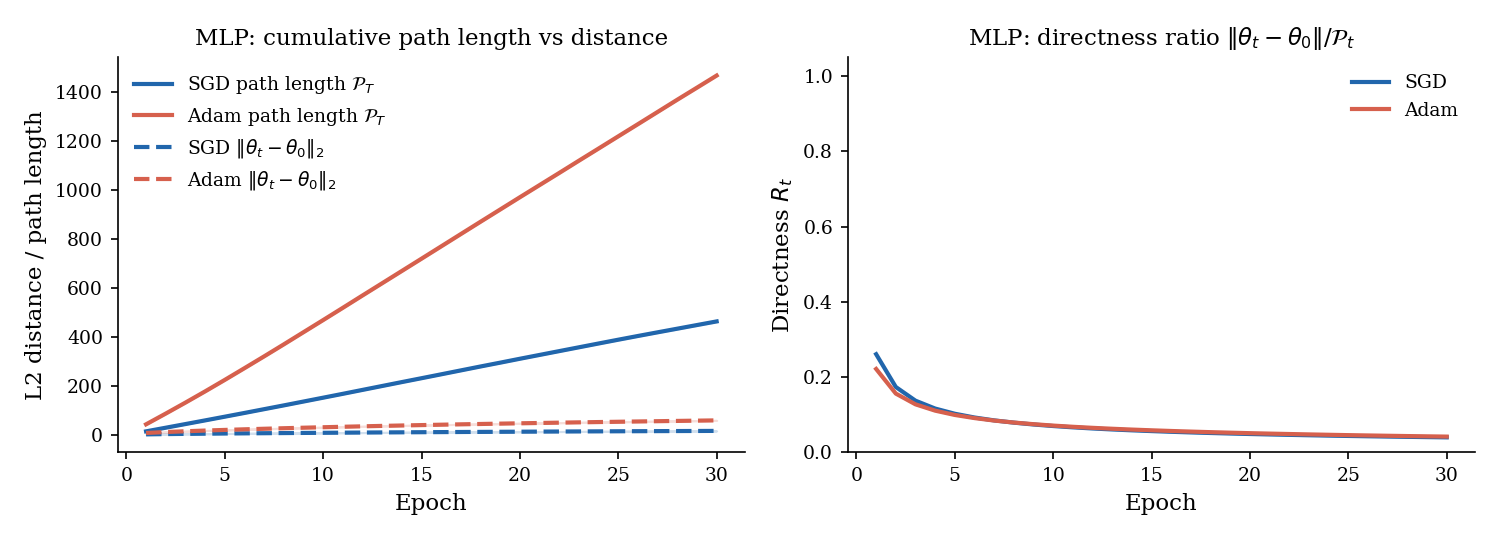
\includegraphics[width=\linewidth]{figures/part2_geometry/path_length_curve_mlp.png}\caption{MLP}\end{subfigure}
\begin{subfigure}{0.48\linewidth}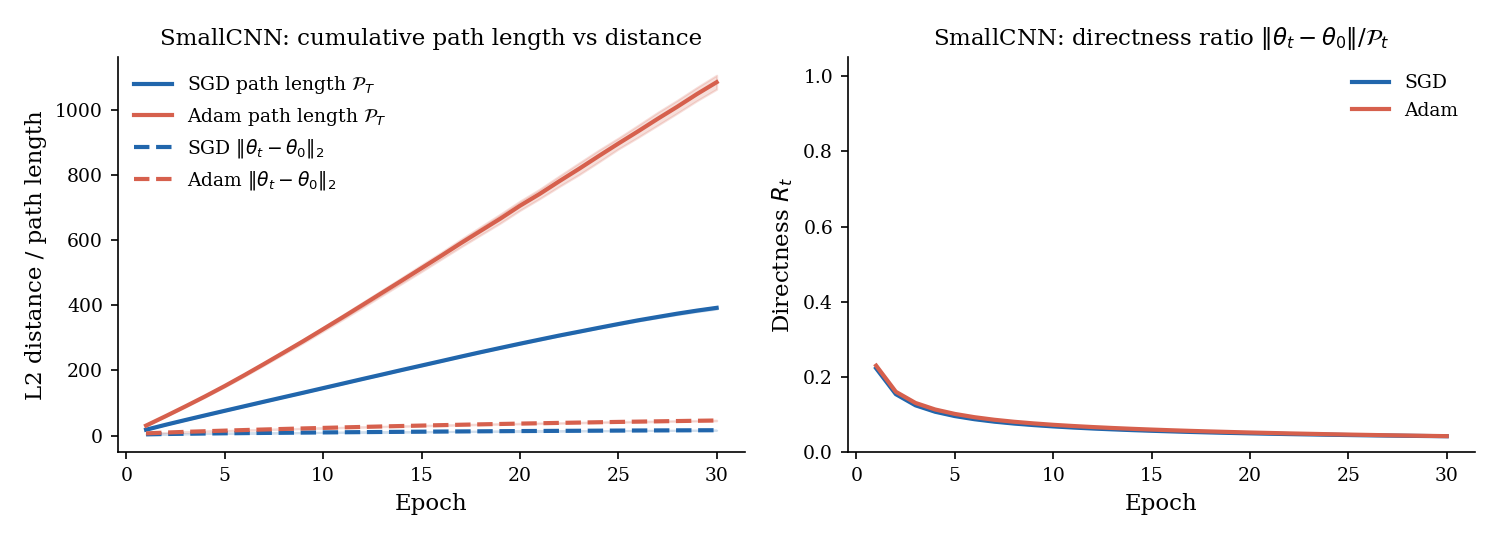
\includegraphics[width=\linewidth]{figures/part2_geometry/path_length_curve_cnn.png}\caption{SmallCNN}\end{subfigure}
\caption{Per-epoch cumulative path length $\mathcal{P}_t$ versus net displacement $\|\theta_t-\theta_0\|_2$. Mean over five matched seeds; bands are $\pm 1$ std. Adam's path length grows much faster than its endpoint distance, so the bigger gap is in step size, not direction.}
\label{fig:path-length}
\end{figure}

\begin{figure}[H]
\centering
\begin{subfigure}{0.48\linewidth}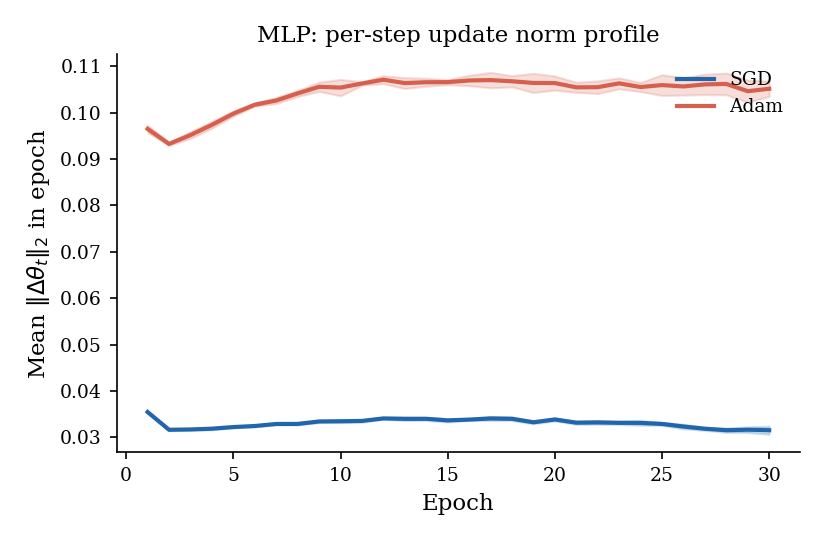
\includegraphics[width=\linewidth]{figures/part2_geometry/step_norm_curve_mlp.png}\caption{MLP}\end{subfigure}
\begin{subfigure}{0.48\linewidth}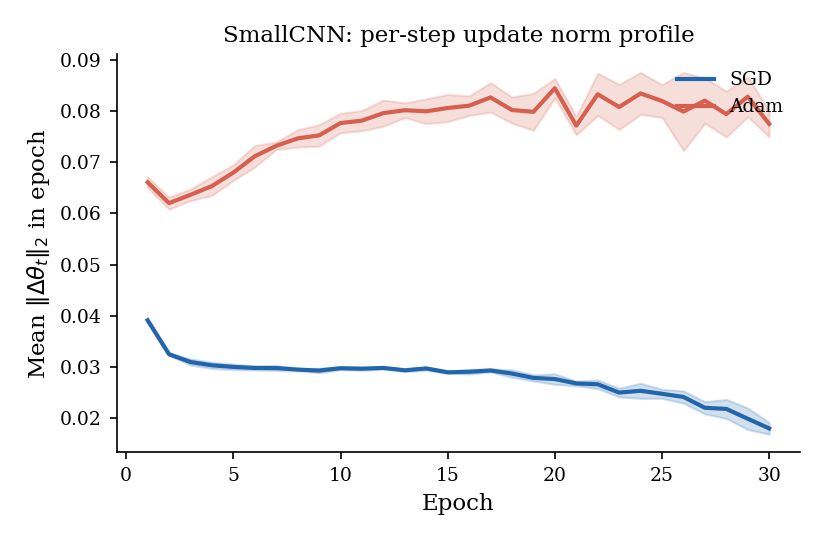
\includegraphics[width=\linewidth]{figures/part2_geometry/step_norm_curve_cnn.png}\caption{SmallCNN}\end{subfigure}
\caption{Mean per-step update norm $\overline{\|\Delta\theta_t\|}_2$ by epoch, five matched seeds.}
\label{fig:step-norm}
\end{figure}

\FloatBarrier

\subsection{Sharpness and Hessian Trace}
\label{sec:hessian}

We compute two Hessian-based proxies at the final epoch on a fixed mini-batch of $512$ examples in evaluation mode.

\paragraph{Sharpness $\lambda_{\max}$ via power iteration.}
Starting from a random unit vector $v_0$, we iterate
\[
  v_{k+1} = \frac{H(\hat\theta)\,v_k}{\|H(\hat\theta)\,v_k\|_2},
  \qquad
  \lambda_{\max} \approx v_k^\top H(\hat\theta)\,v_k,
\]
stopping when $|\lambda_k - \lambda_{k-1}| < 10^{-4}$ or after $100$ iterations.
The Hessian-vector product $H(\hat\theta)v$ is computed without materializing $H$ using second-order automatic differentiation (Pearlmutter's trick):
\[
  H(\hat\theta)\,v = \nabla_\theta\!\left[\nabla_\theta \widehat{L}(\hat\theta)^\top v\right].
\]

\paragraph{Hessian trace $\operatorname{tr}(H)$ via Hutchinson's estimator.}
For $m = 30$ independent Rademacher vectors $z^{(i)} \sim \{\pm 1\}^d$,
\[
  \operatorname{tr}(H) = \mathbb{E}\bigl[z^\top H z\bigr]
  \approx \frac{1}{m}\sum_{i=1}^{m} \bigl(z^{(i)}\bigr)^\top H(\hat\theta)\,z^{(i)}.
\]
The Hutchinson identity follows from $\mathbb{E}[zz^\top]=I$ for Rademacher vectors:
\[
\mathbb{E}[z^\top H z]
=
\mathbb{E}[\operatorname{tr}(z^\top H z)]
=
\mathbb{E}[\operatorname{tr}(Hzz^\top)]
=
\operatorname{tr}(H).
\]
The two proxies are complementary: $\lambda_{\max}$ identifies the single worst direction, while $\operatorname{tr}(H)$ aggregates curvature across all directions.

\begin{table}[H]
\centering
\small
\setlength{\tabcolsep}{4pt}
\begin{tabular}{llccccc}
\toprule
\textbf{Model} & \textbf{Opt.} & \textbf{Test acc.} & \textbf{Gap} & \textbf{$\lambda_{\max}(H)$} & \textbf{$\operatorname{tr}(H)$} & \textbf{Param dist.}\\
\midrule
MLP      & SGD  & $0.8901 \pm 0.0024$ & $0.0904 \pm 0.0027$ & $36.20 \pm 5.97$  & $409.71 \pm 30.44$ & $18.49 \pm 0.03$\\
MLP      & Adam & $0.8887 \pm 0.0030$ & $0.0912 \pm 0.0026$ & $7.22 \pm 1.34$   & $68.13 \pm 5.04$   & $61.20 \pm 0.15$\\
\midrule
SmallCNN & SGD  & $0.9166 \pm 0.0010$ & $0.0779 \pm 0.0028$ & $42.58 \pm 15.71$ & $242.47 \pm 50.04$ & $16.75 \pm 0.09$\\
SmallCNN & Adam & $0.9150 \pm 0.0009$ & $0.0780 \pm 0.0030$ & $64.17 \pm 13.88$ & $218.91 \pm 61.41$ & $46.79 \pm 0.94$\\
\bottomrule
\end{tabular}
\caption{Final scalar metrics across five matched seeds (mean $\pm$ std). Accuracy and gap are reported as fractions. Gap $=$ train accuracy $-$ test accuracy.}
\label{tab:q2_scalars}
\end{table}

\begin{figure}[H]
\centering
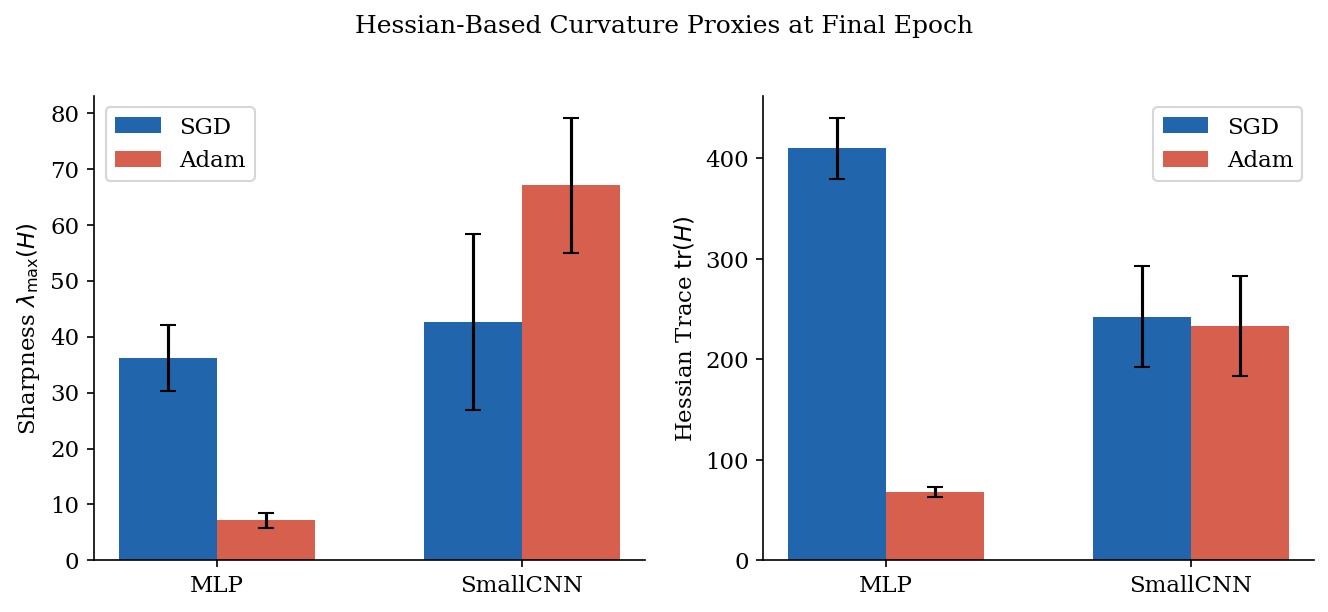
\includegraphics[width=\linewidth]{figures/part2_geometry/sharpness_trace.png}
\caption{Hessian-based curvature proxies at the final epoch.
  \emph{Left}: dominant eigenvalue $\lambda_{\max}(H)$. \emph{Right}: Hessian trace $\operatorname{tr}(H)$.
  Error bars show $\pm 1$ std across five seeds.
  The MLP shows a clear separation: Adam is substantially flatter on both measures.
  In the SmallCNN, Adam's $\lambda_{\max}$ is \emph{higher} than SGD's, while the traces are comparable.}
\label{fig:sharpness}
\end{figure}

\paragraph{MLP.}
The difference is large and consistent across all five seeds.
SGD reaches solutions with $\lambda_{\max} = 36.20 \pm 5.97$ and trace $409.71 \pm 30.44$, while Adam reaches $\lambda_{\max} = 7.22 \pm 1.34$ and trace $68.13 \pm 5.04$.
Adam's solutions are $5\times$ flatter in dominant eigenvalue and $6\times$ lower in total curvature; the error bars of the two optimizers do not overlap in either metric.

The MLP result also clarifies the relationship between distance from initialization and sharpness: Adam travels $3.3\times$ farther yet ends in a much flatter region.
This pattern is plausible geometrically: a long journey can end in a broad valley, while a short journey can end near a narrow basin.
In our experiment, the latter pattern describes SGD: it remains close to $\theta_0$ but arrives in a sharper region.

\paragraph{SmallCNN.}
The CNN result runs in the opposite direction for $\lambda_{\max}$: Adam's mean dominant eigenvalue ($64.17 \pm 13.88$) is higher than SGD's ($42.58 \pm 15.71$), while the Hessian traces are comparable ($218.91$ vs.\ $242.47$, a difference smaller than one standard deviation).
So the CNN case cannot be summarized as simply ``Adam is flatter'' or ``SGD is flatter.''
The architecture's inductive bias from convolutional weight sharing and pooling appears to constrain both optimizers to regions of comparable overall curvature.

\subsection{Perturbation Flatness}
\label{sec:perturbation}

The Hessian-based proxies in Section~\ref{sec:hessian} are local quadratic measurements. To test whether they reflect actual loss robustness, we now evaluate the loss change under explicit parameter perturbations. The local quadratic approximation predicts
\[
\widehat L(\theta^\star+\delta) - \widehat L(\theta^\star)
\approx \frac{1}{2}\,\delta^\top H(\theta^\star)\,\delta,
\]
and for isotropic $\delta\sim\mathcal{N}(0,\sigma^2 I)$,
\[
\mathbb{E}_{\delta}\big[\widehat L(\theta^\star+\delta)-\widehat L(\theta^\star)\big]
\approx \tfrac{\sigma^2}{2}\operatorname{tr}(H).
\]

\paragraph{Relative global perturbation.}
To make perturbation magnitudes comparable across optimizers whose absolute parameter scales differ (Adam typically reaches points with larger $\|\theta\|_2$), we use a \emph{relative} global perturbation:
\[
\delta = \sigma\,\frac{\|\theta^\star\|_2}{\|\xi\|_2}\,\xi,
\qquad \xi\sim\mathcal{N}(0,I_d).
\]
Equivalently, $\|\delta\|_2 = \sigma\,\|\theta^\star\|_2$, so $\sigma$ controls the ratio of perturbation norm to parameter norm. We sweep $\sigma\in\{10^{-4},3\times 10^{-4},10^{-3},3\times 10^{-3},10^{-2}\}$ and average over $K=10$ independent perturbations per $\sigma$. Loss is evaluated on a fixed subset of $4096$ training examples in evaluation mode (BatchNorm running stats from training).

\paragraph{Results.} Figure~\ref{fig:perturbation} shows $\Delta\widehat L(\sigma)$ versus $\sigma$ on log--log axes for both architectures and both optimizers.

\begin{figure}[H]
\centering
\begin{subfigure}{0.48\linewidth}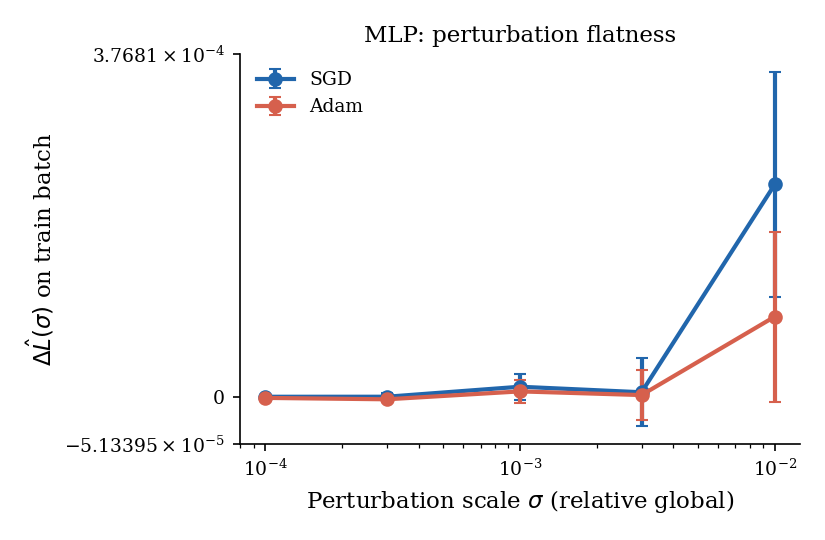
\includegraphics[width=\linewidth]{figures/part2_geometry/perturbation_curve_mlp.png}\caption{MLP}\end{subfigure}
\begin{subfigure}{0.48\linewidth}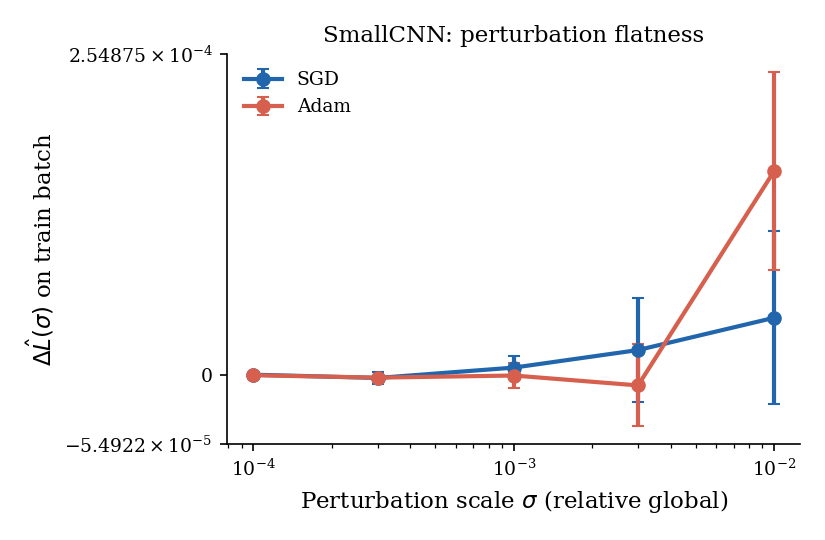
\includegraphics[width=\linewidth]{figures/part2_geometry/perturbation_curve_cnn.png}\caption{SmallCNN}\end{subfigure}
\caption{Mean training-loss increase $\Delta\widehat L(\sigma)$ under relative isotropic Gaussian perturbations, averaged over five matched seeds and $K=10$ perturbations per $\sigma$. Values at $\sigma \le 3\times 10^{-3}$ are at the noise floor ($\le 10^{-5}$); the operational comparison is at $\sigma=10^{-2}$.}
\label{fig:perturbation}
\end{figure}

Across $\sigma \in \{10^{-4}, 3\!\times\!10^{-4}, 10^{-3}, 3\!\times\!10^{-3}\}$, $\Delta\widehat L$ is at the $\le 10^{-5}$ level for all four (architecture, optimizer) configurations and is statistically indistinguishable from zero given the seed variability; these data points primarily establish a noise floor. We therefore restrict the operational comparison to the largest probed magnitude, $\sigma = 10^{-2}$. On the MLP, $\Delta\widehat L = (2.3\pm 1.2)\times 10^{-4}$ for SGD versus $(0.9\pm 0.9)\times 10^{-4}$ for Adam, a $\sim 2.5\times$ gap in the direction predicted by the trace ratio in Section~\ref{sec:hessian}; the seed standard deviations are well separated from zero for both optimizers. On the SmallCNN, the values are $(0.5\pm 0.7)\times 10^{-4}$ for SGD and $(1.6\pm 0.8)\times 10^{-4}$ for Adam: the central tendency is in the same direction as the Hessian and loss-matched $\lambda_{\max}$ readings, but both seed standard deviations overlap zero, so this is a directional observation from $N=5$ seeds rather than a statistically significant reversal. The perturbation evidence corroborates the Hessian readings only at the operational $\sigma = 10^{-2}$ contrast, and only on the MLP at one-sigma confidence.

\FloatBarrier

\subsection{Inter-Seed Parameter Dispersion}
\label{sec:dispersion}

We measure the reproducibility of each optimizer's solutions by computing the mean pairwise L2 distance over all $\binom{5}{2} = 10$ pairs of final parameter vectors:
\[
  \bar{d} = \frac{1}{\binom{5}{2}} \sum_{i < j} \|\hat\theta^*_i - \hat\theta^*_j\|_2.
\]

\begin{table}[H]
\centering
\begin{tabular}{lcc}
\toprule
\textbf{Architecture} & \textbf{SGD mean pairwise dist.} & \textbf{Adam mean pairwise dist.}\\
\midrule
MLP      & $31.50$ & $87.72$\\
SmallCNN & $27.04$ & $67.33$\\
\bottomrule
\end{tabular}
\caption{Inter-seed parameter dispersion. Adam produces more dispersed final parameter vectors across seeds in both architectures.}
\label{tab:interseed}
\end{table}

\begin{figure}[H]
\centering
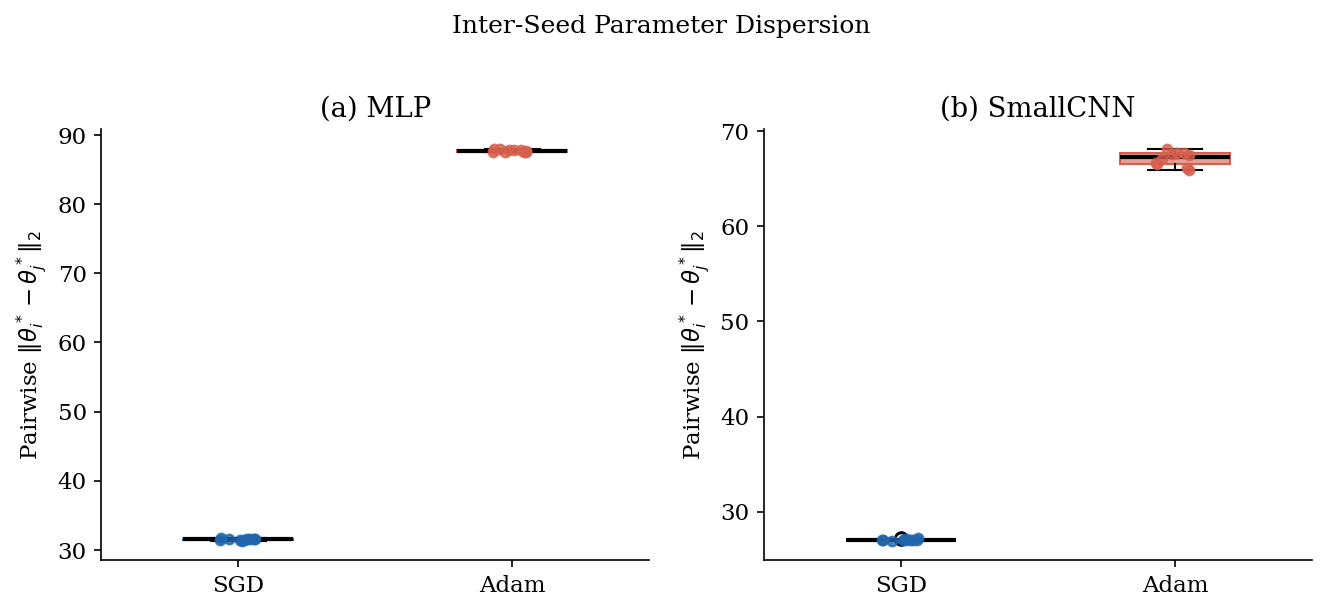
\includegraphics[width=\linewidth]{figures/part2_geometry/inter_seed.png}
\caption{Inter-seed parameter dispersion.
  Each point is the L2 distance $\|\hat\theta^*_i - \hat\theta^*_j\|_2$ between final parameter vectors of two seeds, for a fixed optimizer.
  SGD points are nearly superimposed in both architectures.
  Adam solutions are $2.8\times$ more dispersed in the MLP and $2.5\times$ more dispersed in the SmallCNN.}
\label{fig:interseed}
\end{figure}

Table~\ref{tab:interseed} and Figure~\ref{fig:interseed} show a consistent pattern across both architectures.
SGD solutions are tightly clustered across seeds (MLP: $31.50$; CNN: $27.04$); in Figure~\ref{fig:interseed}, the dots are nearly superimposed.
Adam solutions are systematically more dispersed: $87.72$ for the MLP ($2.8\times$) and $67.33$ for the CNN ($2.5\times$).
The small spread of the dots within each optimizer means that the pairwise distances are consistent. The main point is that Adam's pairwise distances are consistently much larger than SGD's.

This dispersion pattern appears in both architectures tested, including the SmallCNN where curvature evidence is inconclusive. It therefore suggests that the optimizer effect is not limited to the MLP: Adam is more sensitive to the stochastic trajectory and lands in more separated regions across seeds.
One plausible explanation is Adam's coordinate-wise rescaling: across different seeds, small early differences in initialization and minibatch trajectories may affect coordinates differently, and adaptive normalization can allow these differences to accumulate over training.

\subsection{Loss-Matched Geometry Control}
\label{sec:loss-matched}

\paragraph{Motivation.} Fixed-epoch comparisons can confound geometric differences with differences in training-loss level. If at epoch~30 Adam reaches a smaller training loss than SGD does, then the Hessian and distance values being compared are taken at different points along each optimizer's loss-versus-time curve. A reader could legitimately ask whether the geometric gap is just an artifact of the loss gap. The loss-matched control answers this question and is the most important falsification test for the geometry verdict that the previous five subsections build up.

\paragraph{Method.} For each matched seed and architecture, let $\widehat L_{\mathrm{Adam}}^{\mathrm{final}}$ be the final training loss of Adam at epoch $T$. We then search the SGD trajectory for the epoch
\[
t^\star = \arg\min_{t\in\{1,\dots,T\}} \big| \widehat L_{\mathrm{SGD}}(t) - \widehat L_{\mathrm{Adam}}^{\mathrm{final}}\big|,
\]
load SGD's parameter checkpoint at epoch $t^\star$, and compare its geometry to Adam's final solution. The compared quantities are the same we used above: distance from initialization, dominant Hessian eigenvalue $\lambda_{\max}(H)$, and Hessian trace.

\paragraph{Results.} Table~\ref{tab:loss-matched} reports the loss-matched comparison. The mean matched SGD epoch is $t^\star = 29.8$ for the MLP and $t^\star = 28.8$ for the SmallCNN, indicating that SGD reaches Adam's final loss late in its 30-epoch trajectory in both architectures.

\begin{table}[H]
\centering
\small
\setlength{\tabcolsep}{4pt}
\begin{tabular}{llccc}
\toprule
\textbf{Model} & \textbf{Endpoint} & $\|\theta-\theta_0\|_2$ & $\lambda_{\max}(H)$ & $\operatorname{tr}(H)$ \\
\midrule
MLP      & SGD @ epoch $t^\star$ & $18.42 \pm 0.10$ & $37.15 \pm 11.65$ & $437.2 \pm 24.3$ \\
MLP      & Adam @ epoch $T$      & $61.29 \pm 0.12$ & $6.86 \pm 0.79$   & $68.4 \pm 9.4$  \\
\addlinespace
SmallCNN & SGD @ epoch $t^\star$ & $16.58 \pm 0.24$ & $6.17 \pm 12.34$  & $221.8 \pm 64.9$ \\
SmallCNN & Adam @ epoch $T$      & $46.62 \pm 0.96$ & $61.77 \pm 26.43$ & $184.8 \pm 57.0$ \\
\bottomrule
\end{tabular}
\caption{Loss-matched control: SGD parameters at the epoch with closest training loss to Adam's final loss, paired with Adam's final parameters. Mean $\pm$ std across five matched seeds.}
\label{tab:loss-matched}
\end{table}

\paragraph{Estimator variance.}
The standard deviations on $\lambda_{\max}(H)$ in Table~\ref{tab:loss-matched} are large relative to the means, particularly for the SmallCNN/SGD entry ($6.17 \pm 12.34$). Two sources of noise compound here: power-iteration estimates on a $\sim 10^5$-parameter neural Hessian are sensitive to the random initialization of the iterate, and the value of $\lambda_{\max}$ itself varies across the five matched seeds. We report mean $\pm$ std for comparability with the rest of Part~II rather than median/IQR. The MLP architecture comparison ($37.15$ vs.\ $6.86$) is statistically distinguishable at one sigma despite this noise, but the SmallCNN reversal ($6.17$ vs.\ $61.77$) should be read as a directional finding from a single architecture pair rather than a tight quantitative claim.

The architecture comparison is striking. On the MLP, Adam's $\lambda_{\max}$ is roughly $5.4\times$ smaller than SGD's at matched training loss ($6.86$ vs.\ $37.15$), and its Hessian trace is $6.4\times$ smaller ($68.4$ vs.\ $437.2$): the flatness gap from Section~\ref{sec:hessian} survives the loss-matching control intact. The two optimizers genuinely select different curvature regimes; Adam's flatter landscape on the MLP is not a consequence of having simply reached lower training loss. On the SmallCNN, the picture inverts: Adam's $\lambda_{\max}$ is roughly $10\times$ \emph{larger} than SGD's at matched loss ($61.77$ vs.\ $6.17$), while Hessian trace is comparable ($184.8$ vs.\ $221.8$). The opposite sign of the curvature gap on the SmallCNN, even after loss matching, suggests that the optimizer-induced flatness ordering is not a universal property of Adam-versus-SGD: at least one of these architecture-optimizer combinations produces a different selection. Given the single architecture pair and the high variance of $\lambda_{\max}$ estimates noted above, we read this as a directional finding that motivates replication on a larger architecture sample rather than as an established architectural rule.

Function-space disagreement also persists at matched loss. At $t^\star$ versus $T$, $D_{\mathrm{pred}}$ is $0.0772 \pm 0.0066$ on the MLP and $0.0692 \pm 0.0024$ on the SmallCNN, while symmetric KL is $0.1880$ and $0.2858$ respectively---values comparable to the standard final-epoch comparison reported in Section~\ref{sec:function-space}. Even after controlling for training progress, SGD and Adam have selected different predictors.

\FloatBarrier

\subsection{Part~II Synthesis}
\label{sec:part2-synthesis}

The six measurements converge on a coherent geometry verdict. Adam moves substantially farther from initialization in both architectures, and the trajectory decomposition shows the larger displacement is driven by larger per-step updates rather than by a more directed walk. On the MLP, Hessian sharpness and trace, perturbation flatness at the operational scale, and the loss-matched control all agree that Adam selects markedly flatter solutions; on the SmallCNN, the Hessian and loss-matched evidence point in the opposite direction for $\lambda_{\max}$, while perturbation flatness gives a directional but not statistically significant reading. Inter-seed parameter dispersion shows that Adam's solutions are systematically less reproducible across seeds in both architectures, indicating that the optimizer effect is not limited to the MLP. The loss-matched control rules out the most natural alternative explanation: at matched training loss, the MLP flatness gap and the cross-optimizer function-space disagreement both persist.

The most important caveat from Part~II is, however, that the MLP's flatness advantage for Adam does \emph{not} translate into a generalization advantage: test accuracy is marginally lower for Adam ($88.87\%$ vs.\ $89.01\%$) and the train--test gap is marginally larger ($9.12\%$ vs.\ $9.04\%$), with both differences inside the seed-to-seed standard deviation. This is the central tension that Part~III now investigates: a multi-faceted Part~II shows the geometry differs, but Part~III asks whether the differences propagate to predictions.

\FloatBarrier

\section{Part III: Generalization and the Propagation of Implicit Bias}
\label{sec:part3}

\subsection{From Geometry to Generalization: Why More Levels Are Needed}

Part~II establishes that Adam and SGD select geometrically distinct parameter regions in a way that cannot be explained as simply ``Adam reaches lower training loss faster.'' The third project question now asks whether this difference matters for generalization. The straightforward measurement --- final test accuracy and train--test gap --- gives a negative answer at this protocol scale, and on the MLP it does so in the direction \emph{opposite} to a simple flat-minima account: Adam reaches solutions $5\times$ flatter in $\lambda_{\max}$ but slightly worse on test accuracy.

A negative generalization result with a positive parameter-geometry result is the central puzzle of this project, and it is what motivates the rest of Part~III. If the parameter-space difference is real but does not show up in test accuracy, then somewhere along the chain ``parameters $\to$ basin $\to$ predictor $\to$ representation $\to$ test loss'' the optimizer signal must be compressing. We therefore organize the rest of Part~III as three further levels of geometry, in increasing distance from raw parameter values:
\begin{enumerate}
\item Basin geometry (Section~\ref{sec:mode-connectivity}): are the two endpoints in the same low-loss basin, or in different ones?
\item Function-space similarity (Section~\ref{sec:function-space}): do the two endpoints realize the same predictor on test inputs?
\item Representation-space alignment (Section~\ref{sec:representation-space}): do they share penultimate-layer features, after the predictor head is removed?
\end{enumerate}
A same-optimizer cross-seed baseline (10 seed pairs per architecture and per optimizer) is added at every level, so that ``optimizer matters'' is tested against the reference scale of ``seed matters''. Section~\ref{sec:three-level} gathers the verdicts into a three-level synthesis. This is not an optional add-on to the generalization question; it is the only way to explain why Part~II's clear parameter-space difference does not become a Part~III generalization difference.

\subsection{Test Accuracy and Sharpness--Gap Relationship}

\begin{table}[H]
\centering
\caption{Final scalar generalization metrics across five matched seeds (mean $\pm$ std). Gap $=$ train accuracy $-$ test accuracy.}
\label{tab:part3-scalar}
\small
\setlength{\tabcolsep}{5pt}
\begin{tabular}{llccc}
\toprule
Model    & Opt. & Test acc.\ (\%)     & Gap (\%)           & $\lambda_{\max}(H)$ \\
\midrule
MLP      & SGD  & $89.01 \pm 0.24$   & $9.04 \pm 0.27$    & $36.20 \pm 5.97$  \\
MLP      & Adam & $88.87 \pm 0.30$   & $9.12 \pm 0.26$    & $7.22  \pm 1.34$  \\
SmallCNN & SGD  & $91.66 \pm 0.10$   & $7.79 \pm 0.28$    & $42.58 \pm 15.71$ \\
SmallCNN & Adam & $91.50 \pm 0.09$   & $7.80 \pm 0.30$    & $64.17 \pm 13.88$ \\
\bottomrule
\end{tabular}
\end{table}

\begin{figure}[H]
  \centering
  \begin{subfigure}{0.48\linewidth}
    \centering
    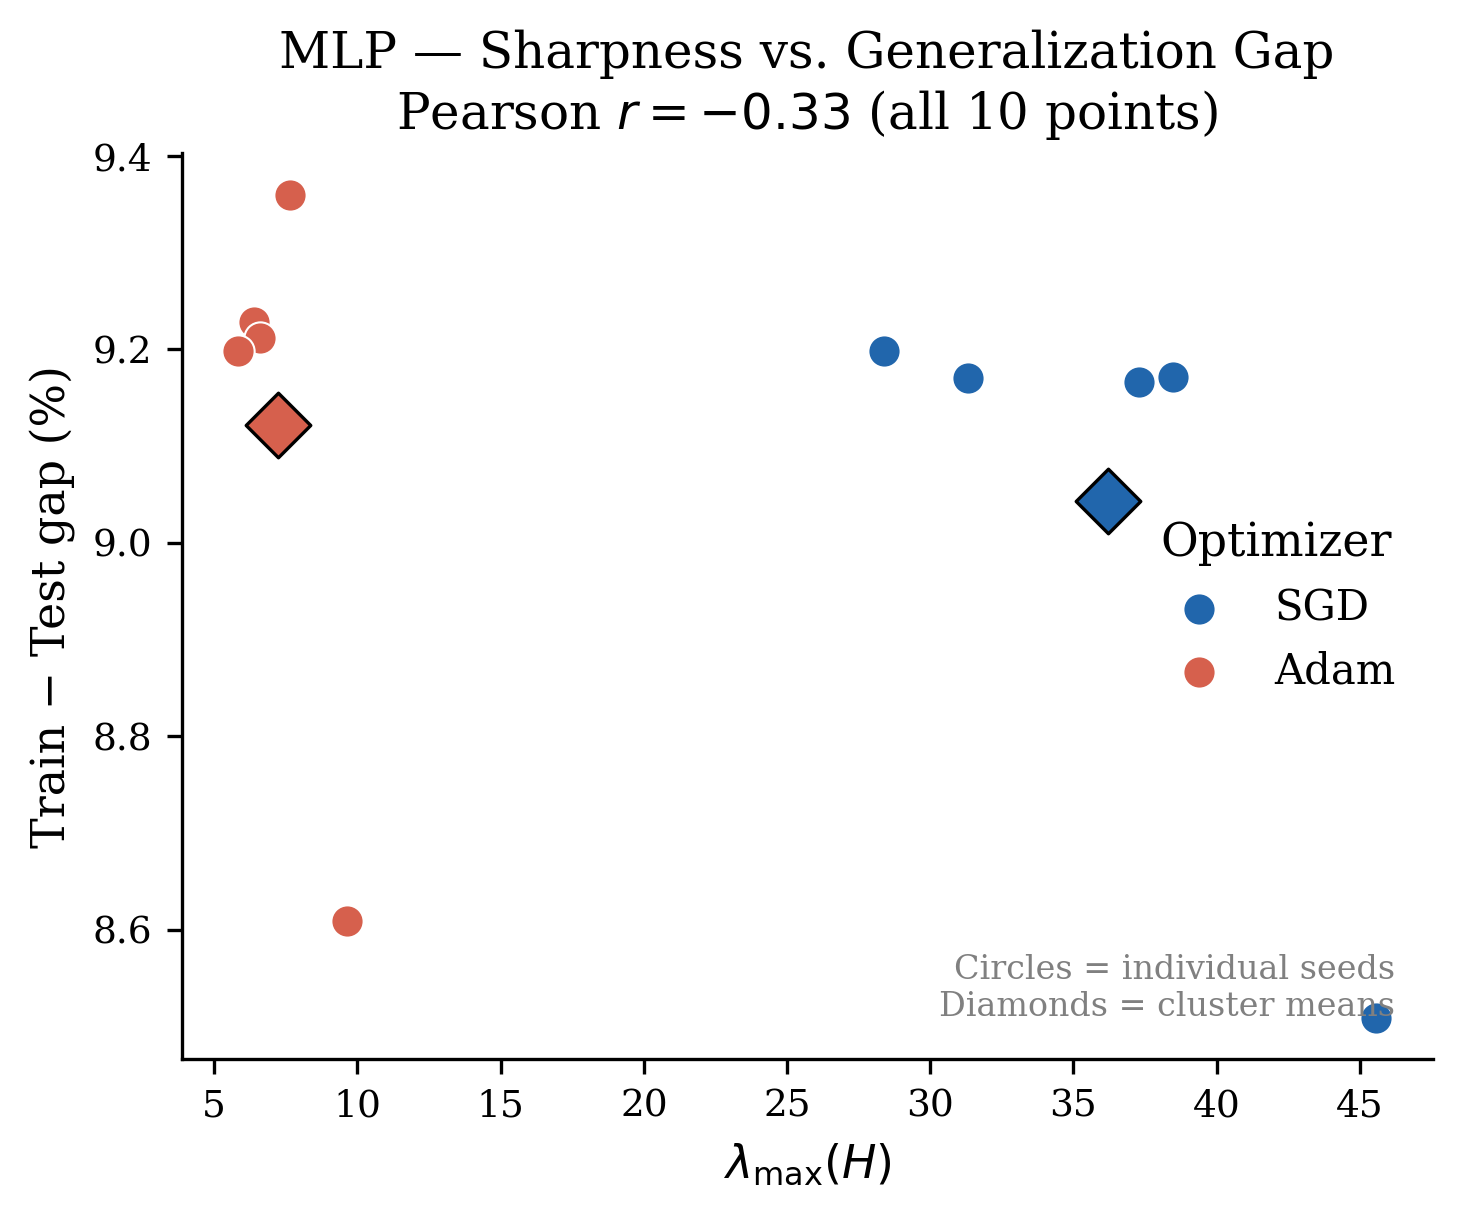
\includegraphics[width=\linewidth]{figures/part3_generalization/sharpness_gap_mlp.png}
    \caption{MLP}
  \end{subfigure}
  \hfill
  \begin{subfigure}{0.48\linewidth}
    \centering
    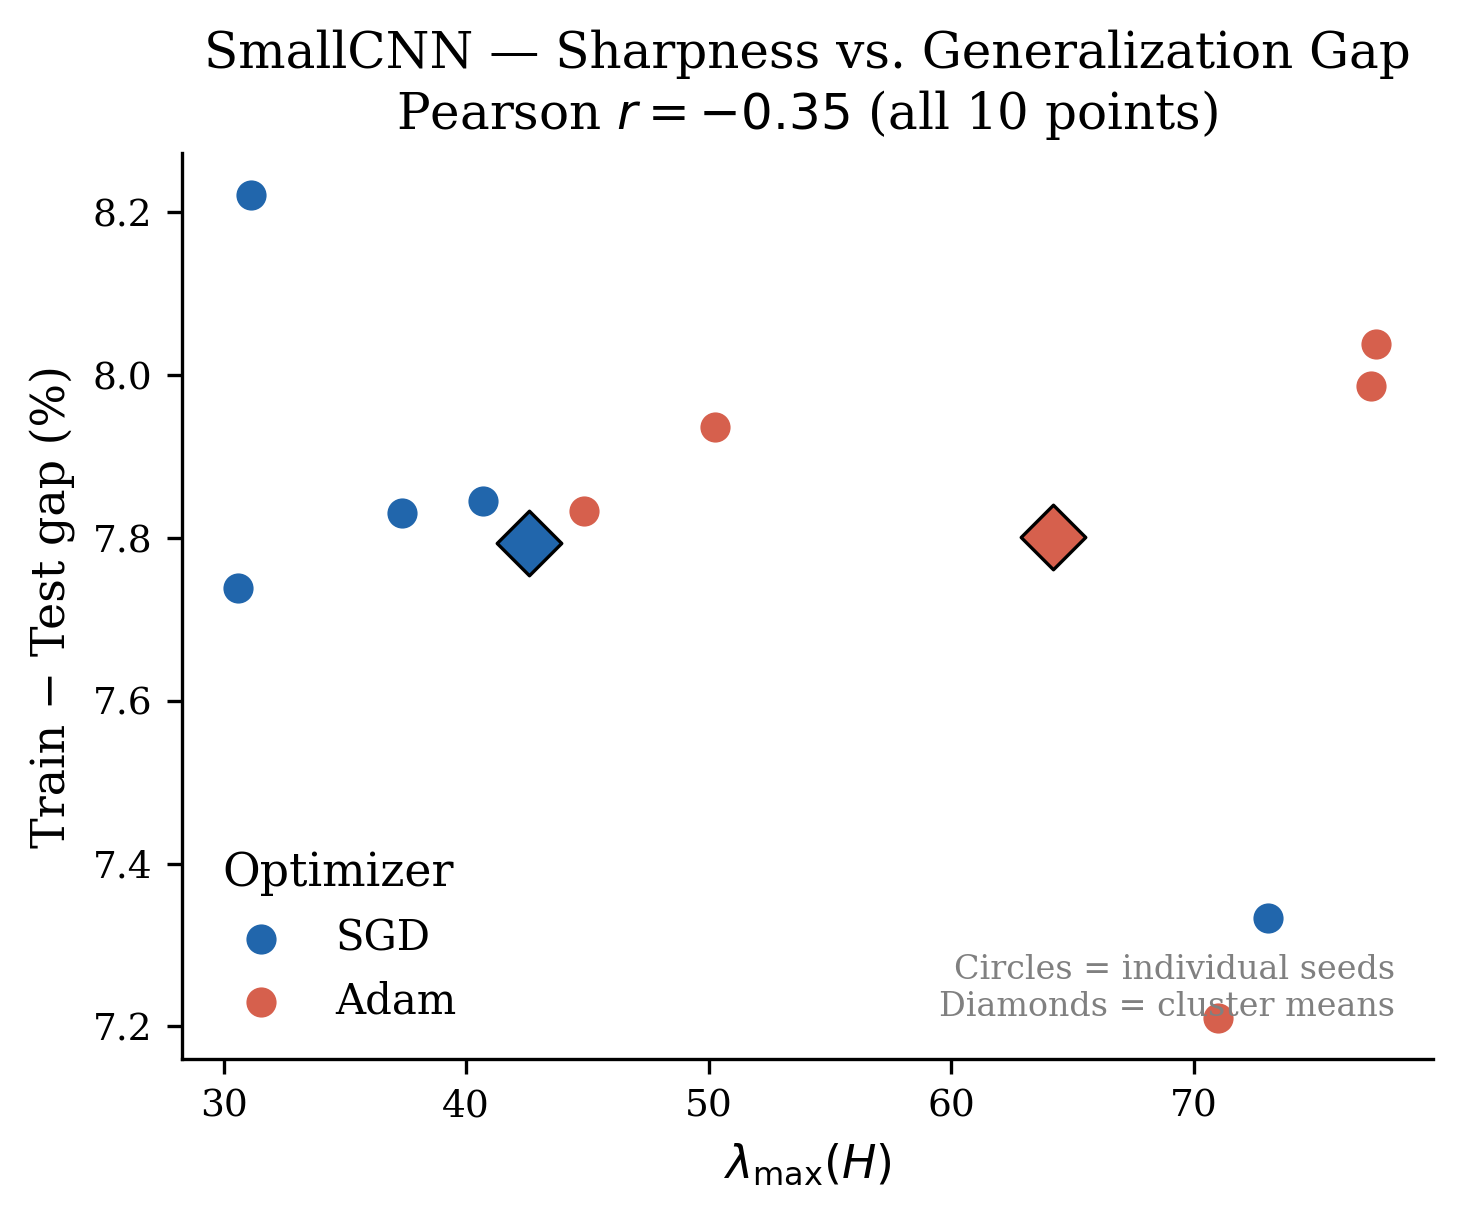
\includegraphics[width=\linewidth]{figures/part3_generalization/sharpness_gap_cnn.png}
    \caption{SmallCNN}
  \end{subfigure}
  \caption{Final-epoch sharpness $\lambda_{\max}(H)$ versus train--test gap. Each marker is one matched-seed run; diamonds are cluster centroids. In the MLP, the optimizer clusters are well-separated in sharpness ($\lambda_{\max}\approx 36$ for SGD vs.\ $\approx 7$ for Adam) but not in gap. In the SmallCNN, the optimizer clusters overlap on both axes.}
  \label{fig:part3-scatter}
\end{figure}

\paragraph{MLP.}
Adam reaches solutions with $\lambda_{\max}=7.22\pm 1.34$ versus SGD's $36.20\pm 5.97$ --- a $5\times$ flatness advantage that simple flat-minima accounts \cite{hochreiter1997flat,keskar2017large} would predict to translate into better generalization. The data point in the opposite direction: SGD has marginally higher test accuracy ($89.01\%$ vs.\ $88.87\%$) and a marginally smaller train--test gap ($9.04\%$ vs.\ $9.12\%$). Both differences are within seed-to-seed standard deviation, so we do not claim a robust ranking, but the direction is striking: lower Euclidean Hessian sharpness here is not associated with any generalization benefit. Figure~\ref{fig:part3-scatter} visualizes this: the two optimizer clusters are widely separated horizontally (sharpness) but vertically overlapping (gap).

\paragraph{SmallCNN.}
Generalization is essentially tied (test accuracy $91.66\%$ vs.\ $91.50\%$; gap $7.79\%$ vs.\ $7.80\%$), and the Hessian ordering is mixed (Adam has higher $\lambda_{\max}$ but comparable trace). The convolutional inductive bias appears to constrain both optimizers to similarly performing solutions even when their parameter trajectories differ.

The combined picture is that the simple flat-minima story is insufficient at this protocol scale. Generalization is mediated by architecture, basin connectivity, function-space behavior, and representation similarity --- the next three subsections probe each in turn.

\FloatBarrier

\subsection{Basin Geometry: Linear Mode Connectivity}
\label{sec:mode-connectivity}

\paragraph{Motivation.} Part~II reports that Adam's solutions are far from SGD's in Euclidean parameter space. A natural follow-up question is whether the two solutions sit in the same low-loss basin or in different basins separated by a loss barrier. Linear mode connectivity \cite{garipov2018loss,frankle2020linear} probes this directly: if a straight-line interpolant between two minima never rises above the larger of their two losses, the minima lie in a connected low-loss region. This is the basin-level analogue of the parameter-space distance reported in Section~\ref{sec:dist}: it converts ``the two optimizers end up far apart in parameter space'' into ``the two endpoints sit in linearly disconnected basins, or not.''

\paragraph{Method.} For each matched seed and architecture, define the line
\[
\theta(\lambda) = (1-\lambda)\,\theta_{\mathrm{SGD}} + \lambda\,\theta_{\mathrm{Adam}},
\qquad \lambda\in\{0,0.1,0.2,\dots,1.0\}.
\]
We evaluate training and test loss at each $\lambda$. For BatchNorm models, the running statistics interpolate to values that no longer match the data, so we recalibrate them at each interior $\lambda$ by a single forward pass over $50$ training batches in train mode (no parameter update). The endpoints $\lambda=0$ and $\lambda=1$ keep their original BN stats. The loss \emph{barrier} is
\[
B = \max_{\lambda\in[0,1]} \widehat L(\theta(\lambda))
   - \max\big\{ \widehat L(\theta_{\mathrm{SGD}}),\; \widehat L(\theta_{\mathrm{Adam}}) \big\}.
\]
$B\approx 0$ indicates linear connectivity; $B>0$ indicates a barrier.

\paragraph{Results.} Figure~\ref{fig:mode-connectivity} plots $\widehat L(\theta(\lambda))$ over the interpolation, and Table~\ref{tab:mode-connectivity} reports $B$ averaged over seeds.

\begin{figure}[H]
\centering
\begin{subfigure}{0.48\linewidth}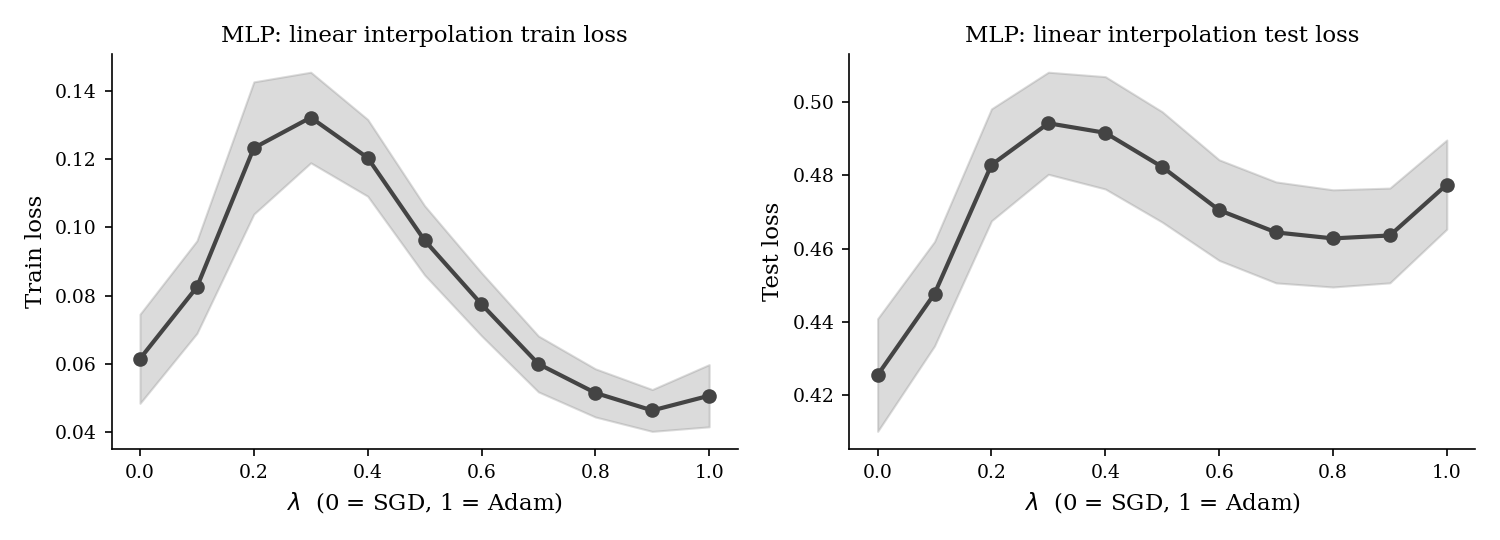
\includegraphics[width=\linewidth]{figures/part3_generalization/mode_connectivity_mlp.png}\caption{MLP}\end{subfigure}
\begin{subfigure}{0.48\linewidth}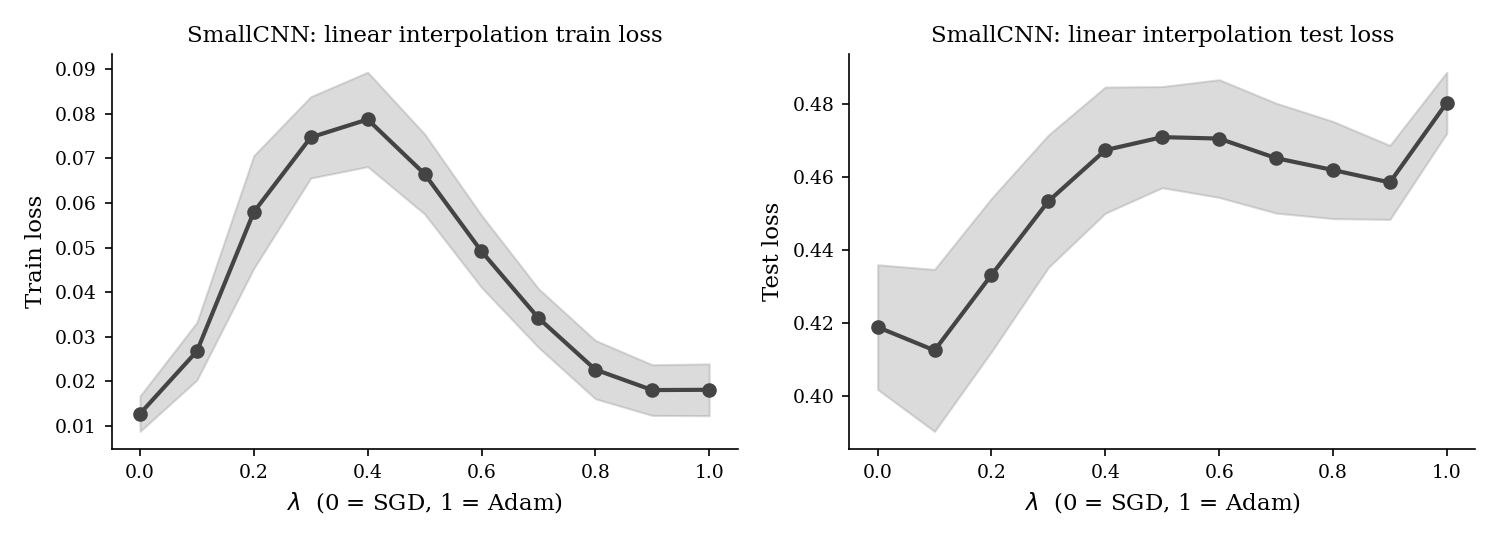
\includegraphics[width=\linewidth]{figures/part3_generalization/mode_connectivity_cnn.png}\caption{SmallCNN}\end{subfigure}
\caption{Linear mode connectivity: training and test loss along $\theta(\lambda)=(1-\lambda)\theta_{\mathrm{SGD}}+\lambda\theta_{\mathrm{Adam}}$, with BatchNorm recalibrated at interior $\lambda$. Solid line is mean over five matched seeds; band is $\pm 1$ std.}
\label{fig:mode-connectivity}
\end{figure}

\begin{table}[H]
\centering
\small
\begin{tabular}{llcc}
\toprule
\textbf{Model} & \textbf{Comparison} & \textbf{Train barrier $B_{\text{train}}$} & \textbf{Test barrier $B_{\text{test}}$} \\
\midrule
MLP      & SGD-vs-Adam (matched seed)   & $0.0721 \pm 0.0086$ & $0.0174 \pm 0.0086$ \\
MLP      & SGD-vs-SGD (cross seed)      & $0.4952 \pm 0.0630$ & $0.2855 \pm 0.0614$ \\
MLP      & Adam-vs-Adam (cross seed)    & $0.4925 \pm 0.0401$ & $0.2528 \pm 0.0389$ \\
\addlinespace
SmallCNN & SGD-vs-Adam (matched seed)   & $0.0615 \pm 0.0078$ & $0.0032 \pm 0.0065$ \\
SmallCNN & SGD-vs-SGD (cross seed)      & $1.1843 \pm 0.2540$ & $0.8102 \pm 0.2547$ \\
SmallCNN & Adam-vs-Adam (cross seed)    & $1.4214 \pm 0.2918$ & $0.9975 \pm 0.2918$ \\
\bottomrule
\end{tabular}
\caption{Loss barrier along the linear interpolation between two trained solutions. Top sub-block per architecture: matched-seed SGD-vs-Adam (mean $\pm$ std over five seeds). Lower sub-blocks: same-optimizer cross-seed baseline averaged over $C(5,2)=10$ seed pairs. The matched-seed cross-optimizer barrier is roughly an order of magnitude smaller than either same-optimizer cross-seed baseline.}
\label{tab:mode-connectivity}
\end{table}

The matched-seed cross-optimizer training-loss barriers are small but consistently positive ($0.0721$ for the MLP, $0.0615$ for the SmallCNN), and substantially larger than the cross-seed standard deviations: there is a real, reproducible bump in training loss along the straight line connecting matched SGD and Adam solutions, even after BatchNorm recalibration. The same-optimizer cross-seed baselines, however, give a far higher barrier scale: $B_{\text{train}}^{\mathrm{SS}} = 0.4952 \pm 0.0630$ and $B_{\text{train}}^{\mathrm{AA}} = 0.4925 \pm 0.0401$ on the MLP, and $1.1843 \pm 0.2540$ / $1.4214 \pm 0.2918$ on the SmallCNN. The cross-optimizer matched-seed barrier is therefore roughly $7\times$ smaller than the same-optimizer cross-seed barrier on the MLP and $\sim 20\times$ smaller on the SmallCNN. The basin separation between SGD and Adam at matched seed is real but, in absolute terms, far smaller than the basin separation between two same-optimizer runs from different initializations. The large same-optimizer cross-seed barrier is consistent with the instability finding of Frankle et al.~\cite{frankle2020linear}: in standard training, two SGD runs that differ only in initialization land in distinct linearly disconnected basins, and our SGD-vs-SGD and Adam-vs-Adam baselines reproduce this effect at our scale. What drives basin connectivity in this protocol is therefore primarily the shared seed (initialization plus minibatch order), not optimizer agreement; the cross-optimizer effect is a small additional barrier on top of an otherwise highly connected matched-seed landscape. Test-loss barriers tell the same story at lower magnitude: $0.0174$ / $0.0032$ for matched-seed cross-optimizer pairs versus $\sim 0.25$--$1.0$ for same-optimizer cross-seed pairs.

\FloatBarrier

\subsection{Function-Space Similarity}
\label{sec:function-space}

\paragraph{Motivation.} Parameter-space distance does not directly measure how different the trained networks are as functions. Two networks can have very different parameter vectors and still produce nearly identical predictions on the data distribution, especially in the presence of scale symmetries and BatchNorm. To check whether the optimizer-induced parameter differences carry through to functional differences, we evaluate three function-level metrics on the test set. This is the predictor-level analogue of Part~II's parameter measurements: it asks whether the parameter difference still exists once we look at outputs rather than weights.

\paragraph{Metrics.} For matched SGD and Adam models with predicted class probabilities $p_S(\cdot|x)$ and $p_A(\cdot|x)$ and pre-softmax logits $z_S(x), z_A(x)$, we compute, over the $N$-point test set:
\begin{align}
D_{\mathrm{pred}} &= \frac{1}{N}\sum_{i=1}^N \mathbf{1}\!\big[\arg\max_k p_S(k|x_i)\ne \arg\max_k p_A(k|x_i)\big],\\
D_{\mathrm{SKL}} &= \frac{1}{2N}\sum_{i=1}^N \big[D_{\mathrm{KL}}(p_S\|p_A) + D_{\mathrm{KL}}(p_A\|p_S)\big],\\
C_{\mathrm{logit}} &= \frac{1}{N}\sum_{i=1}^N \frac{z_S(x_i)^\top z_A(x_i)}{\|z_S(x_i)\|_2\,\|z_A(x_i)\|_2}.
\end{align}
$D_{\mathrm{pred}}$ is a strict decision-level disagreement; $D_{\mathrm{SKL}}$ measures the divergence of the full softmax distribution; $C_{\mathrm{logit}}$ is scale-invariant and captures direction similarity in logit space.

\paragraph{Results.} Table~\ref{tab:function-space} reports the three metrics.

\begin{table}[H]
\centering
\small
\begin{tabular}{llccc}
\toprule
\textbf{Model} & \textbf{Comparison} & $D_{\mathrm{pred}}$ & $D_{\mathrm{SKL}}$ & $C_{\mathrm{logit}}$ \\
\midrule
MLP      & SGD-vs-Adam (matched seed) & $0.0738 \pm 0.0028$ & $0.1749 \pm 0.0051$ & $0.6122 \pm 0.0058$ \\
MLP      & SGD-vs-SGD (cross seed)    & $0.0868 \pm 0.0067$ & $0.2056 \pm 0.0286$ & $0.9187 \pm 0.0035$ \\
MLP      & Adam-vs-Adam (cross seed)  & $0.0822 \pm 0.0042$ & $0.2348 \pm 0.0195$ & $0.9561 \pm 0.0022$ \\
\addlinespace
SmallCNN & SGD-vs-Adam (matched seed) & $0.0671 \pm 0.0042$ & $0.2676 \pm 0.0219$ & $0.6516 \pm 0.0061$ \\
SmallCNN & SGD-vs-SGD (cross seed)    & $0.0740 \pm 0.0045$ & $0.3121 \pm 0.0324$ & $0.9050 \pm 0.0039$ \\
SmallCNN & Adam-vs-Adam (cross seed)  & $0.0786 \pm 0.0031$ & $0.4038 \pm 0.0212$ & $0.9295 \pm 0.0040$ \\
\bottomrule
\end{tabular}
\caption{Function-space similarity on the Fashion-MNIST test set. Top sub-block per architecture: matched-seed SGD-vs-Adam (mean $\pm$ std over five seeds). Lower sub-blocks: same-optimizer cross-seed baseline averaged over $C(5,2)=10$ pairs. $D_{\mathrm{pred}}$ and $D_{\mathrm{SKL}}$ are at or below the same-optimizer cross-seed baseline; only the logit-direction cosine $C_{\mathrm{logit}}$ shows a sharp matched-seed cross-optimizer signal.}
\label{tab:function-space}
\end{table}

The two matched-seed predictors disagree on $7.4\%$ of MLP test predictions and $6.7\%$ of SmallCNN predictions. The same-optimizer cross-seed baselines on $D_{\mathrm{pred}}$ are $0.0868 \pm 0.0067$ (SGD-vs-SGD) and $0.0822 \pm 0.0042$ (Adam-vs-Adam) on the MLP, and $0.0740 \pm 0.0045$ / $0.0786 \pm 0.0031$ on the SmallCNN. The matched-seed cross-optimizer $D_{\mathrm{pred}}$ is therefore at or slightly \emph{below} the same-optimizer cross-seed baseline; symmetric KL behaves the same way ($0.1749$ for cross-optimizer matched seed on the MLP, versus $0.20$--$0.23$ for same-optimizer cross-seed). Decision-level and softmax-level disagreement at this protocol scale is not driven by the choice of optimizer above the level of seed-induced disagreement. The exception is logit-direction cosine: $C_{\mathrm{logit}} \approx 0.61$--$0.65$ between matched SGD and Adam, versus $0.92$--$0.96$ within either optimizer across seeds. Optimizer choice does therefore shift the pre-softmax logit \emph{direction} substantially, but argmax decisions and full softmax distributions absorb most of that shift. The architecture comparison adds a secondary effect: the SmallCNN has slightly lower $D_{\mathrm{pred}}$ but higher $D_{\mathrm{SKL}}$ than the MLP, indicating that when the convolutional models do disagree they tend to disagree more confidently in distribution.

\FloatBarrier
\begin{figure}[H]
\centering
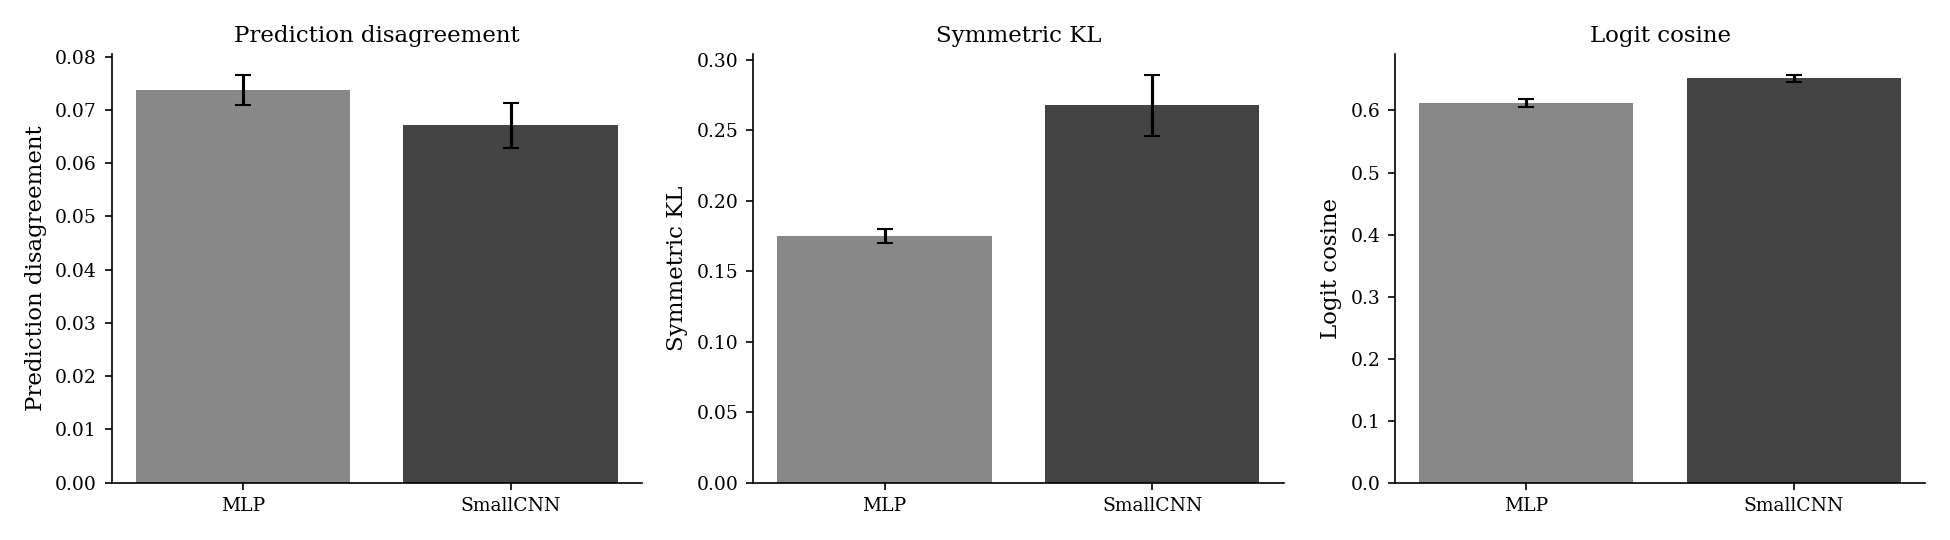
\includegraphics[width=0.6\linewidth]{figures/part3_generalization/function_space_bars.png}
\caption{Function-space disagreement metrics on Fashion-MNIST test set, mean $\pm$ std over five seeds.}
\label{fig:function-space-bars}
\end{figure}

\FloatBarrier

\subsection{Representation-Space Alignment}
\label{sec:representation-space}

Function-space metrics compare outputs, but two models can have similar outputs while using different internal representations. We therefore compare penultimate-layer features using linear centered kernel alignment (CKA) \cite{kornblith2019similarity}. Let $F_S$ and $F_A$ denote centered feature matrices for matched SGD and Adam models on the same test subset. Linear CKA is
\[
\mathrm{CKA}(F_S,F_A)=
\frac{\|F_S^\top F_A\|_F^2}{\|F_S^\top F_S\|_F\,\|F_A^\top F_A\|_F}.
\]
It is insensitive to isotropic rescaling and is a more stable representation-similarity diagnostic than raw feature distance. This is the deepest level in the chain ``parameters $\to$ basin $\to$ predictor $\to$ representation'': it asks whether, after stripping the final classifier head, the two optimizers have built the same internal feature geometry.

\begin{table}[H]
\centering
\small
\begin{tabular}{llcc}
\toprule
\textbf{Model} & \textbf{Comparison} & \textbf{Feature kernel alignment $A$} & \textbf{Linear CKA} \\
\midrule
MLP      & SGD-vs-Adam (matched seed) & $0.9697 \pm 0.0010$ & $0.8578 \pm 0.0059$ \\
MLP      & SGD-vs-SGD (cross seed)    & $0.9698 \pm 0.0008$ & $0.8613 \pm 0.0038$ \\
MLP      & Adam-vs-Adam (cross seed)  & $0.9714 \pm 0.0008$ & $0.8497 \pm 0.0071$ \\
\addlinespace
SmallCNN & SGD-vs-Adam (matched seed) & $0.9664 \pm 0.0027$ & $0.9147 \pm 0.0113$ \\
SmallCNN & SGD-vs-SGD (cross seed)    & $0.9774 \pm 0.0006$ & $0.9220 \pm 0.0033$ \\
SmallCNN & Adam-vs-Adam (cross seed)  & $0.9677 \pm 0.0024$ & $0.8920 \pm 0.0107$ \\
\bottomrule
\end{tabular}
\caption{Representation-space alignment between penultimate-layer features. Matched cross-optimizer values are close to same-optimizer cross-seed baselines, suggesting that optimizer choice does not strongly reshape representation geometry at this protocol scale.}
\label{tab:representation}
\end{table}

The key result is that representation similarity remains high. Matched SGD-vs-Adam CKA is $0.858$ for the MLP and $0.915$ for the SmallCNN, close to the corresponding same-optimizer cross-seed baselines. Thus the large parameter-space separation does not become a large representation-space separation. Combined with the function-space results, this suggests a layered effect: optimizer choice strongly changes parameter trajectories, moderately changes logit directions, but only weakly changes penultimate feature geometry. The negative generalization result of Section~\ref{sec:part3}'s opening is therefore consistent: the parameter-level signal compresses substantially before reaching the predictor and representation levels at which test accuracy is determined.

\FloatBarrier

\subsection{Three-Level Synthesis: Parameter, Basin, Function--Representation}
\label{sec:three-level}

The whole Part~II / Part~III sequence is now organized around three levels of geometry, summarized in Table~\ref{tab:three-level}.

\begin{table}[H]
\centering
\small
\setlength{\tabcolsep}{3pt}
\begin{tabular}{p{2.4cm}p{4.8cm}p{4.5cm}p{3.5cm}}
\toprule
\textbf{Level} & \textbf{Quantities} & \textbf{What it answers} & \textbf{Verdict (this study)} \\
\midrule
Parameter geometry (Part~II) & $\|\theta_T-\theta_0\|_2$, $\mathcal{P}_T$, $R_T$, $\lambda_{\max}(H)$, $\operatorname{tr}(H)$, $\bar d_{\mathrm{seed}}$, $\Delta\widehat L(\sigma)$ & Where does the optimizer go, and what is the local curvature? & Adam path length $\sim 3\times$ SGD's in both architectures; directness ratio essentially equal. MLP: Adam $\sim 5$--$6\times$ flatter at matched loss. SmallCNN: ordering may reverse, but this is a single-architecture-pair observation with high $\lambda_{\max}$ estimator variance. \\
\addlinespace
Basin geometry (Part~III) & Linear-interpolation loss curve, barrier $B$ & Are the two solutions in the same low-loss region? & Cross-optimizer matched-seed train barrier ($0.072$ MLP, $0.062$ CNN) is $\sim 7\times$--$20\times$ smaller than the same-optimizer cross-seed baseline ($0.49$ MLP, $1.18$--$1.42$ CNN). The matched-seed protocol drives connectivity; cross-optimizer adds a small additional barrier. Test barrier $\le 0.02$ for matched-seed pairs. \\
\addlinespace
Function and representation geometry (Part~III) & $D_{\mathrm{pred}}$, $D_{\mathrm{SKL}}$, $C_{\mathrm{logit}}$, $A(K_S,K_A)$, CKA & Do parameter differences correspond to different predictors or representations? & $D_{\mathrm{pred}}$ ($\sim 7\%$) and CKA ($0.86$--$0.91$) are within the same-optimizer cross-seed baseline range; only $C_{\mathrm{logit}}\approx 0.6$ (vs.\ $0.92$--$0.96$ within-optimizer) shows a sharp matched-seed cross-optimizer signal. Optimizer choice reshapes logit direction but not argmax decisions or representation geometry beyond seed noise at this scale. \\
\bottomrule
\end{tabular}
\caption{Three-level synthesis of the implicit-bias evidence.}
\label{tab:three-level}
\end{table}

The data, with the same-optimizer cross-seed baseline added, support the following conservative version of the message we anticipated:
\begin{quote}
\emph{Adam substantially changes parameter-space trajectory and local Euclidean geometry on the MLP, and the change survives the loss-matching control. As the comparison propagates from parameters to predictions, however, much of what looked like a cross-optimizer effect compresses to within the same-optimizer cross-seed baseline: $D_{\mathrm{pred}}$, $D_{\mathrm{SKL}}$, $A$, and linear CKA on matched-seed cross-optimizer pairs lie within the range observed between two runs of the same optimizer at different seeds. The matched-seed protocol drives basin connectivity an order of magnitude beyond what shared-optimizer cross-seed pairs achieve; the cross-optimizer matched-seed train barrier is small but nonzero, and the only function-level metric that shows a sharp cross-optimizer signal above seed noise is the logit-direction cosine $C_{\mathrm{logit}}$. Architecture mediates which curvature regime each optimizer selects, but the SmallCNN flatness reversal is a single-architecture-pair observation with high $\lambda_{\max}$ estimator variance and should be replicated.}
\end{quote}

This is the core message of the project. Optimizer-induced parameter geometry is real, especially on the MLP, and not merely a final-loss artifact; but with a same-optimizer cross-seed baseline in view, the function- and representation-level differences between matched SGD and Adam at this protocol scale are mostly accounted for by seed-induced variability rather than by optimizer-induced bias, with $C_{\mathrm{logit}}$ as the principal exception.

\FloatBarrier


\section{Overall Discussion}

The main question was whether adaptive optimization alters implicit bias and generalization. The answer is layered. Adam clearly changes parameter-space trajectory: it moves farther from initialization, travels a longer path, and produces more dispersed endpoints. On the MLP, this difference remains visible after loss matching and appears in much lower Hessian curvature and smaller perturbation loss increase. On the CNN, the curvature ordering is less stable, which suggests that architecture can dominate or redirect optimizer-induced geometry.

The effect becomes weaker as we move away from parameters. Linear mode connectivity shows that matched SGD and Adam endpoints are not simply identical points in the same basin, but their train-loss barrier is much smaller than same-optimizer cross-seed barriers. Function-space metrics show nontrivial logit-direction differences, yet prediction disagreement and symmetric KL remain close to same-optimizer cross-seed baselines. Representation CKA is even more compressed: penultimate features remain highly aligned across optimizers. The most concise summary is therefore:
\begin{quote}
\emph{Adam changes geometry strongly in parameter space, mildly in basin and logit geometry, and weakly in representation geometry.}
\end{quote}
This explains why the generalization story is not binary. The MLP shows the strongest flatness advantage for Adam, but Adam does not obtain a clear test-accuracy or gap advantage. The CNN shows similar generalization even when parameter trajectories differ. The conclusion direction is consistent with Wilson et al.~\cite{wilson2017marginal}, who report that adaptive methods can generalize worse than well-tuned SGD; the underlying mechanism in our MLP setting is, however, the opposite of the one they invoke: they attribute the gap to Adam selecting \emph{sharper} minima, whereas in our matched-seed Fashion-MNIST MLP Adam selects substantially \emph{flatter} solutions and still does not generalize better. Thus optimizer-induced implicit bias is real, but its effect on test performance is filtered through architecture, loss level, basin connectivity, functional equivalence, and representation similarity.

\subsection{Scale-Aware Sharpness and Reparameterization Caveat}
\label{sec:normalized-sharpness}

The Hessian quantities in this report are Euclidean parameter-space diagnostics. They are useful for controlled within-architecture comparisons, but not invariant measures of function complexity. For a two-layer ReLU network,
\[
f(x)=W_2\sigma(W_1x),
\]
positive homogeneity gives
\[
W_2\sigma(W_1x)=(c^{-1}W_2)\sigma(cW_1x),\qquad c>0.
\]
The two parameterizations represent the same function but can have different norms and Hessian spectra. BatchNorm introduces related scale freedoms. This reparameterization caveat \cite{dinh2017sharp} is why we interpret $\lambda_{\max}(H)$, $\operatorname{tr}(H)$, and perturbation flatness as within-protocol diagnostics rather than universal generalization measures.

\subsection{Limitations}
\label{sec:limitations}

The study uses one dataset, two small architectures, five seeds, and finite hyperparameter tuning. Hessian estimates are mini-batch proxies, and BatchNorm complicates both sharpness and mode-connectivity interpretation. The no-regularization protocol is useful for isolating optimizer effects, but it is not a production training recipe. The architecture-dependent flatness reversal should therefore be interpreted as a directional observation worth replicating, not as a universal Adam-vs-SGD law.

\section{Conclusion}

This project compared SGD with momentum and Adam as two preconditioned stochastic dynamics, and structured the entire investigation around three linked questions: convergence, solution geometry, and generalization. The central mathematical distinction is that SGD uses scalar spatial preconditioning, while Adam uses a time-varying diagonal preconditioner, leading locally to different error dynamics through
\[
e_{t+1}\approx (I-P_tH)e_t.
\]
Empirically, the geometry question is answered with six complementary measurements (distance, path length and update norm, Hessian sharpness/trace, perturbation flatness, inter-seed dispersion, loss-matched control), and they jointly show that Adam selects different parameter-space regions under matched seeds in a way that is not merely an artifact of training-loss level. The generalization question is then answered by following the parameter-space difference through three further levels of geometry --- basin, function, and representation --- and finds that the optimizer signal compresses substantially as it propagates: matched-seed cross-optimizer basin barriers are an order of magnitude smaller than same-optimizer cross-seed barriers, prediction disagreement and CKA fall within the same-optimizer cross-seed baseline, and only logit-direction cosine still shows a sharp cross-optimizer signal. The final lesson is therefore not that Adam or SGD is universally better, but that adaptive preconditioning changes solution selection while generalization depends on how that parameter-space change survives through architecture, basin structure, function space, and representation geometry.

\begin{thebibliography}{9}

\bibitem{kingma2015adam}
Diederik P. Kingma and Jimmy Ba.
\newblock Adam: A Method for Stochastic Optimization.
\newblock International Conference on Learning Representations, 2015.
\newblock \url{https://arxiv.org/abs/1412.6980}.

\bibitem{hochreiter1997flat}
Sepp Hochreiter and J\"urgen Schmidhuber.
\newblock Flat Minima.
\newblock Neural Computation, 9(1):1--42, 1997.
\newblock \url{https://doi.org/10.1162/neco.1997.9.1.1}.

\bibitem{keskar2017large}
Nitish Shirish Keskar, Dheevatsa Mudigere, Jorge Nocedal, Mikhail Smelyanskiy, and Ping Tak Peter Tang.
\newblock On Large-Batch Training for Deep Learning: Generalization Gap and Sharp Minima.
\newblock International Conference on Learning Representations, 2017.
\newblock \url{https://openreview.net/forum?id=H1oyRlYgg}.

\bibitem{dinh2017sharp}
Laurent Dinh, Razvan Pascanu, Samy Bengio, and Yoshua Bengio.
\newblock Sharp Minima Can Generalize For Deep Nets.
\newblock International Conference on Machine Learning, 2017.
\newblock \url{https://proceedings.mlr.press/v70/dinh17b.html}.

\bibitem{wilson2017marginal}
Ashia C. Wilson, Rebecca Roelofs, Mitchell Stern, Nati Srebro, and Benjamin Recht.
\newblock The Marginal Value of Adaptive Gradient Methods in Machine Learning.
\newblock Advances in Neural Information Processing Systems, 2017.
\newblock \url{https://proceedings.neurips.cc/paper/2017/hash/81b3833e2504647f9d794f7d7b9bf341-Abstract.html}.

\bibitem{garipov2018loss}
Timur Garipov, Pavel Izmailov, Dmitrii Podoprikhin, Dmitry P. Vetrov, and Andrew Gordon Wilson.
\newblock Loss Surfaces, Mode Connectivity, and Fast Ensembling of DNNs.
\newblock Advances in Neural Information Processing Systems, 2018.
\newblock \url{https://proceedings.neurips.cc/paper/2018/hash/be3087e74e9100d4bc4c6268cdbe8456-Abstract.html}.

\bibitem{frankle2020linear}
Jonathan Frankle, Gintare Karolina Dziugaite, Daniel M. Roy, and Michael Carbin.
\newblock Linear Mode Connectivity and the Lottery Ticket Hypothesis.
\newblock International Conference on Machine Learning, 2020.
\newblock \url{https://proceedings.mlr.press/v119/frankle20a.html}.

\bibitem{kornblith2019similarity}
Simon Kornblith, Mohammad Norouzi, Honglak Lee, and Geoffrey Hinton.
\newblock Similarity of Neural Network Representations Revisited.
\newblock International Conference on Machine Learning, 2019.
\newblock \url{https://proceedings.mlr.press/v97/kornblith19a.html}.

\end{thebibliography}

\end{document}
